%%
%% This is file `sample-sigconf.tex',
%% generated with the docstrip utility.
%%
%% The original source files were:
%%
%% samples.dtx  (with options: `all,proceedings,bibtex,sigconf')
%% 
%% IMPORTANT NOTICE:
%% 
%% For the copyright see the source file.
%% 
%% Any modified versions of this file must be renamed
%% with new filenames distinct from sample-sigconf.tex.
%% 
%% For distribution of the original source see the terms
%% for copying and modification in the file samples.dtx.
%% 
%% This generated file may be distributed as long as the
%% original source files, as listed above, are part of the
%% same distribution. (The sources need not necessarily be
%% in the same archive or directory.)
%%
%%
%% Commands for TeXCount
%TC:macro \cite [option:text,text]
%TC:macro \citep [option:text,text]
%TC:macro \citet [option:text,text]
%TC:envir table 0 1
%TC:envir table* 0 1
%TC:envir tabular [ignore] word
%TC:envir displaymath 0 word
%TC:envir math 0 word
%TC:envir comment 0 0
%%
%% The first command in your LaTeX source must be the \documentclass
%% command.
%%
%% For submission and review of your manuscript please change the
%% command to \documentclass[manuscript, screen, review]{acmart}.
%%
%% When submitting camera ready or to TAPS, please change the command
%% to \documentclass[sigconf]{acmart} or whichever template is required
%% for your publication.
%%
%%
\documentclass[sigconf]{acmart}
%%
%% \BibTeX command to typeset BibTeX logo in the docs
% \AtBeginDocument{%
%   \providecommand\BibTeX{{%
%     Bib\TeX}}}

%% Rights management information.  This information is sent to you
%% when you complete the rights form.  These commands have SAMPLE
%% values in them; it is your responsibility as an author to replace
%% the commands and values with those provided to you when you
%% complete the rights form.
% \setcopyright{acmlicensed}
\setcopyright{none}
% \copyrightyear{2018}
% \acmYear{2018}
% \acmDOI{XXXXXXX.XXXXXXX}
%% These commands are for a PROCEEDINGS abstract or paper.
% \acmConference[Conference acronym 'XX]{Make sure to enter the correct
%   conference title from your rights confirmation email}{June 03--05,
%   2018}{Woodstock, NY}
%%
%%  Uncomment \acmBooktitle if the title of the proceedings is different
%%  from ``Proceedings of ...''!
%%
%%\acmBooktitle{Woodstock '18: ACM Symposium on Neural Gaze Detection,
%%  June 03--05, 2018, Woodstock, NY}
% \acmISBN{978-1-4503-XXXX-X/2018/06}
\acmConference{CSCI6806 Capstone Proj}{Fall 2025}{Vancouver, BC, CA}

\settopmatter{printacmref=false,printfolios=true} % removes the footnote below the first column
\renewcommand\footnotetextcopyrightpermission[1]{} % removes conference info footnote

%%
%% Submission ID.
%% Use this when submitting an article to a sponsored event. You'll
%% receive a unique submission ID from the organizers
%% of the event, and this ID should be used as the parameter to this command.
%%\acmSubmissionID{123-A56-BU3}

%%
%% For managing citations, it is recommended to use bibliography
%% files in BibTeX format.
%%
%% You can then either use BibTeX with the ACM-Reference-Format style,
%% or BibLaTeX with the acmnumeric or acmauthoryear sytles, that include
%% support for advanced citation of software artefact from the
%% biblatex-software package, also separately available on CTAN.
%%
%% Look at the sample-*-biblatex.tex files for templates showcasing
%% the biblatex styles.
%%

%%
%% The majority of ACM publications use numbered citations and
%% references.  The command \citestyle{authoryear} switches to the
%% "author year" style.
%%
%% If you are preparing content for an event
%% sponsored by ACM SIGGRAPH, you must use the "author year" style of
%% citations and references.
%% Uncommenting
%% the next command will enable that style.
%%\citestyle{acmauthoryear}

% fix figure
\usepackage{array}
\usepackage{adjustbox}

\usepackage[inkscapelatex=false]{svg}
\svgsetup{inkscapelatex=false}

\usepackage{graphicx}
\usepackage{subcaption} % современная замена subfig
\usepackage{float}
\usepackage{makecell}

% use placeins with float barrier to fix position of fig 4a 4b 4c 4d
% \usepackage{placeins}

% use labelfont, labelsep for removing ":" to fix caption of 4a 4b 4c 4d
% \usepackage[labelfont=bf,labelsep=none]{caption}

%%
%% end of the preamble, start of the body of the document source.
\begin{document}

%%
%% The "title" command has an optional parameter,
%% allowing the author to define a "short title" to be used in page headers.
\title{Group 1: Study on Baleen Flash Caches}

%%
%% The "author" command and its associated commands are used to define
%% the authors and their affiliations.
%% Of note is the shared affiliation of the first two authors, and the
%% "authornote" and "authornotemark" commands
%% used to denote shared contribution to the research.

\vfill
\author{Anna Gorislavets}
\affiliation{%
  \institution{Fairleigh Dickinson University}
  \city{Vancouver}
  \country{Canada}
  }
\email{a.gorislavets@student.fdu.edu}

\author{Bikash Shyangtang}
\affiliation{%
  \institution{Fairleigh Dickinson University}
  \city{Vancouver}
  \country{Canada}
  }
\email{b.shyangtang@student.fdu.edu}

\author{Hao Chen}
\affiliation{%
  \institution{Fairleigh Dickinson University}
  \city{Vancouver}
  \country{Canada}
  }
\email{h.chen4@student.fdu.edu}

\author{Maoting Li}
\affiliation{%
  \institution{Fairleigh Dickinson University}
  \city{Vancouver}
  \country{Canada}
  }
\email{m.li3@student.fdu.edu}

\author{Salinrat Thanathapsakun}
\affiliation{%
  \institution{Fairleigh Dickinson University}
  \city{Vancouver}
  \country{Canada}
  }
\email{s.thanathapsakun@student.fdu.edu}

\vfill

%%
%% By default, the full list of authors will be used in the page
%% headers. Often, this list is too long, and will overlap
%% other information printed in the page headers. This command allows
%% the author to define a more concise list
%% of authors' names for this purpose.
% \renewcommand{\shortauthors}{Trovato et al.}

%%
%% The abstract is a short summary of the work to be presented in the
%% article.
\begin{abstract}

This work investigates the impact of varying key parameters in the Baleen flash caching system on performance. Baleen is a machine learning (ML)-based system that determines what data to store in flash memory for faster access and minimizing unnecessary writes. Three key parameters play an important role in the analysis of this work: Dynamic Threshold (\(\tau_{DT}\)), which represents a tunable threshold that dynamically adjusts caching admission or eviction based on data access patterns; the Protected Capacity (PROTECTED Cap), which defines the fraction of cache space reserved for frequently reused data; and Alpha Time-To-Idle (\(\alpha_{tti}\)), which controls how quickly cached entries are considered inactive. This study examines these three parameters under two eviction policies: the Dynamic-Threshold Segmented Least Recently Used (DT-SLRU) and Eviction Decision Engine (EDE), in terms of their impact on system peak Disk-head Time (Peak DT) and cache efficiency (Hit Rate). 

The results demonstrated that the medium value of \(\tau_{DT}\) (namely, 0.001–0.01), for which maximum performance was obtained, led to an optimal delay time of 31.5~ms, with the hit rate reaching approximately 2\%. Both other parameters, PROTECTED Cap and \(\alpha_{tti}\), affect the system only slightly and help stabilize the system in all tested cases. Summing up, Baleen's ML-based strategy performs more efficiently and consistently than standard cache policies with less tuning, indicating that minimal tuning is enough to achieve stable and reliable results.

\end{abstract}

% \pagenumbering{arabic}
% \thispagestyle{empty}

%%
%% The code below is generated by the tool at http://dl.acm.org/ccs.cfm.
%% Please copy and paste the code instead of the example below.
%%
% \begin{CCSXML}
% <ccs2012>
%  <concept>
%   <concept_id>00000000.0000000.0000000</concept_id>
%   <concept_desc>Do Not Use This Code, Generate the Correct Terms for Your Paper</concept_desc>
%   <concept_significance>500</concept_significance>
%  </concept>
%  <concept>
%   <concept_id>00000000.00000000.00000000</concept_id>
%   <concept_desc>Do Not Use This Code, Generate the Correct Terms for Your Paper</concept_desc>
%   <concept_significance>300</concept_significance>
%  </concept>
%  <concept>
%   <concept_id>00000000.00000000.00000000</concept_id>
%   <concept_desc>Do Not Use This Code, Generate the Correct Terms for Your Paper</concept_desc>
%   <concept_significance>100</concept_significance>
%  </concept>
%  <concept>
%   <concept_id>00000000.00000000.00000000</concept_id>
%   <concept_desc>Do Not Use This Code, Generate the Correct Terms for Your Paper</concept_desc>
%   <concept_significance>100</concept_significance>
%  </concept>
% </ccs2012>
% \end{CCSXML}

% \ccsdesc[500]{Do Not Use This Code~Generate the Correct Terms for Your Paper}
% \ccsdesc[300]{Do Not Use This Code~Generate the Correct Terms for Your Paper}
% \ccsdesc{Do Not Use This Code~Generate the Correct Terms for Your Paper}
% \ccsdesc[100]{Do Not Use This Code~Generate the Correct Terms for Your Paper}

%%
%% Keywords. The author(s) should pick words that accurately describe
%% the work being presented. Separate the keywords with commas.
% \keywords{Flash Cache, HDD throughput bottleneck, Disk-head Time (DT)}
%% A "teaser" image appears between the author and affiliation
%% information and the body of the document, and typically spans the
%% page.
% \begin{teaserfigure}
%   \includegraphics[width=\textwidth]{sampleteaser}
%   \caption{Seattle Mariners at Spring Training, 2010.}
%   \Description{Enjoying the baseball game from the third-base
%   seats. Ichiro Suzuki preparing to bat.}
%   \label{fig:teaser}
% \end{teaserfigure}

% \received{20 February 2007}
% \received[revised]{12 March 2009}
% \received[accepted]{5 June 2009}

%%
%% This command processes the author and affiliation and title
%% information and builds the first part of the formatted document.
\maketitle

% \onecolumn make the document one column

% Abstract/Introduction/Conclusion
\clearpage

\section{Introduction}
Modern data centers are confronted with the challenges of managing the performance and cost of two types of storage devices: namely, hard drives (HDDs) that provide bulk storage capacity affordably at the expense of sacrificing efficiency, and solid-state drives (SSDs) to serve as flash cache to absorb peak I/O workloads that wear out quickly if used frequently. Flash cache is capable of improving the system performance significantly by reducing backend request latency; however, it also introduces additional challenges in device wearout optimization that traditional caching policies struggle to effectively address. The center of the problem arises due to the limited write endurance of SSDs, which makes caching every I/O miss indiscriminately infeasible because it would wear out SSDs too quickly and add significant additional cost to large datacenters. The limited write endurance of SSDs necessitates the implementation of admission and eviction policies that intelligently decide which memory block should be written to the flash cache to maximize performance while minimizing flash wearout and reducing backend load. 

Recent research has offered valuable solutions to address this challenge. The Baleen article has illustrated that traditional cache admission and eviction policies, such as hit rate and byte miss rate, fail to capture the real cost of ownership of backend storage. 

%It argues that this is especially true in large data centers. 

The authors proposed that DT, the time that a disk head spends serving backend requests, is in fact a more accurate measure for researchers to capture system performance in large data centers. 
The Baleen article reveals that Peak DT is directly correlated with storage capacity requirements and long-term infrastructure costs. Thus, the minimization of Peak DT is crucial for performance optimization and cost reduction \cite{wong2024baleen}. Likewise, Kangaroo's work shows that conventional heuristic-based cache admission and eviction policies tend to make less than optimal decisions by prioritizing hit rates over system efficiency in the long run \cite{mcallister2021kangaroo}. 

%This leads to under-utilization of system resources and increased operational costs in the long run. 

Existing solutions that aim at optimizing flash caching often have significant limitations. Policies such as Least Recently Used (LRU) and First-In-First-Out (FIFO) evict memory blocks solely based on the order of arrival or recency. This kind of approach ignores the varying potential that each memory block has for system performance. Improved policies like RejectX resort to evaluating each memory block's characteristics on a case-by-case basis; however, RejectX relies on heuristics to make admission and eviction decisions, and therefore, it cannot adapt to varying backend workloads. 
DT-SLRU represents an improvement from RejectX by the integration of service-time considerations; however, its decision-making is still based on heuristics and cannot predict a memory block's reusability reliably. Furthermore, both RejectX and DT-SLRU have a common limitation as both policies treat admission and evictions as two isolated events rather than an integrated segment which can be seen from the episode model in the Baleen article \cite{wong2024baleen}.

%The episode model introduced in the Baleen article treats each cache residency as a single unit (episode) that reflects the true cost of admission in the flash cache more precisely than the traditional metrics based on hit rates. The episode model recognizes periods of active access and idle periods to related memory blocks and makes a prediction on when items will become idle by understanding episode boundaries. Because of this, the episode model makes more informed decisions on which items to retain and which to evict.
%
Concretely, the implementation of the EDE eviction policy focuses on the following three areas. The first one is \(\tau_{DT}\), which admits a memory block only if the admitted block's service-time saving justifies the flash cache it consumes. The second is a PROTECTED Cap, a protected segment that occupies a fixed fraction of the flash cache; the segment therefore prevents useful blocks from premature eviction during their reuse window. The last is the \(\alpha_{tti}\). By making the time-to-idle window adjustable, the protection of around a block naturally expires as the reuse likelihood diminishes. 
%Together, these three modifications align with Baleen's objective of minimizing Peak DT and reducing write amplification, which makes the approach different from earlier heuristics-based policies that focused on hit-rate maximization. With no less than 5 points and 3 runs per point (i.e., Admit-All, prefetch off, normalized reporting), the episode-based policy consistently demonstrates that it is capable of reducing service time and Peak DT when compared to the baseline. 

Furthermore, flash writes are lowered while median latency remains unchanged across all experiments. Comparison between  E0 (LRU), E1 (DT-SLRU), and E2 (EDE) was taken at the given cache size under Admit-All and Prefetch Disabled conditions, reporting Peak DT, median DT, and hit rate each with normalized values; here again, E2 always decreases Peak DT and latency while flash writes were also reduced. This suggests that paying close attention to blocks that have a high reuse potential is more worthwhile than focusing on the median across the entire cache residency. 

The ablation study varied one parameter at a time: $\tau_{DT}$, the PROTECTED Cap, and $\alpha_{\text{tti}}$. The results show that tightening $\tau_{DT}$ reduces flash-cache writes while keeping median latency unchanged. The PROTECTED Cap has little impact on backend load for this workload, whereas a moderate $\alpha_{\text{tti}}$ value ($\approx 0.4$–$0.6$) provides the best balance, lowering Peak DT and tail latency without increasing write amplification.

The project implemented an episode-aware eviction mechanism that treats cache residency as an episode with a deadline linked to $\tau_{DT}$, enabling evaluation of service-time reduction without modifying the core policy logic. The work also introduced a tail-aligned evaluation approach, focusing on Peak DT and service time rather than hit rate, and reporting results for E0 (LRU), E1 (DT-SLRU), and E2 (EDE). Normalized outcomes were presented to support consistent comparisons across different configurations. In addition, ablation-ready controls were developed by varying $\tau_{\text{DT}}$, PROTECTED Cap, and $\alpha_{\text{tti}}$ to analyze each parameter's influence on eviction behavior. The results were documented through original figures containing five or more data points, with variance between runs accounted for under the fixed Admit-All and Prefetch-Disabled conditions.

%Each experiment was executed under identical runtime conditions to preserve reproducibility and consistency with the Baleen artifact methodology. Configuration logs and normalized outputs were retained to verify parameter sensitivity and ensure that observed variations stem solely from controlled changes in $\tau_{\text{DT}}$, PROTECTED Cap, and $\alpha_{\text{tti}}$.

\subsection{Contribution}

\begin{itemize}
  \item \textbf{Provided an extension of Baleen’s eviction evaluation:} The study uses the Baleen-FAST’24 artifact and BCacheSim to reproduce the results illustrated in the Baleen article and modifies the eviction policies by implementing comparisons between the following eviction policies: LRU (E0), DT-SLRU (E1), and EDE (E2) on the Baleen Tectonic trace files, with an emphasis on Peak DT, median DT, and hit rate.
  
  \item \textbf{Parameter isolation and ablation study:} The study isolates key parameters for each eviction policy mentioned above—namely $\tau_{\text{DT}}$, PROTECTED cap, and $\alpha_{\text{tti}}$—to investigate their impact on eviction behavior. The conclusions illustrate strong $\tau_{\text{DT}}$ sensitivity in DT-SLRU and limited sensitivity in EDE.
  
  \item \textbf{Detailed analysis of cache size and backend utilization:} The study analyzes how Peak DT and backend utilization are jointly influenced by both cache size and eviction logic, showing that increasing cache capacity is not sufficient to compensate for poor eviction logic.
  
  \item \textbf{Original scripts and fully reproducible figures:} The study includes configuration files and runnable scripts to enable full reproducibility of all figures presented in the report.
\end{itemize}



\clearpage

\section{Background}

\subsection{Flash Cache \& Disk-head Time}

The Disk-head Time (DT) is a system metric to measure the backend workload of HDDs. It is defined as the time it takes for the disk head to serve a backend request.

The backend load is calculated by adding up the DT of all cache misses over a given time period, and then the sum is divided by the number of disks. The calculation shows how much of the disk capacity across all disks is being used and whether the backend is saturated as a whole \cite{wong2024baleen}.

%figure
\begin{figure}[ht!]
  \centering
  % ACM recommends PDF/EPS/PNG over SVG
  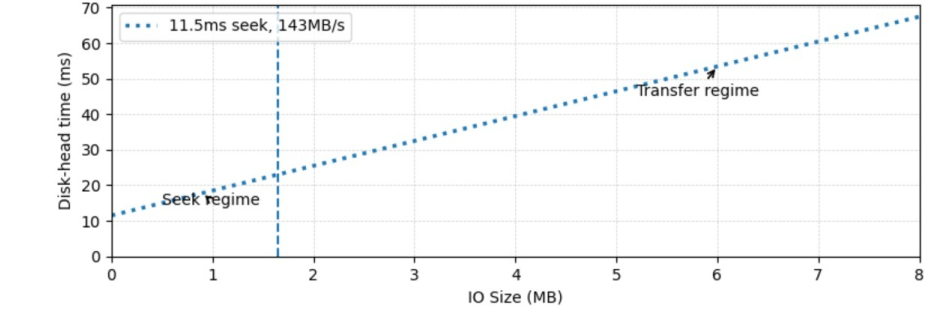
\includegraphics[width=0.50\textwidth]{a1_diagrams/CSCI6806_dt_vs_io.pdf}
  \caption{DT vs I/O size. The dotted line indicates the DT curve. The vertical dotted line denotes the transition from the seek regime for small I/Os to the transfer regime when the I/Os are larger.}
  \label{fig:dt-vs-io}
\end{figure}

Knowing the DT is crucial for large-scale storage systems because system capacity is determined by Peak DT, not hit rates. Data centers rely primarily on HDDs for cost-effectiveness; however, HDDs are limited by throughput. It can only handle about 100 IOPS per disk. When DT exceeds the system capacity, requests get queued up and tail latency increases, and together adversely impact user experience.

Flash caches are incorporated into data storage facilities to accelerate the backend requests by keeping frequently requested or nearby blocks in flash so that repeated requests for access can be served from flash without having to reach for the HDDs (Figure~\ref{fig:2}). The flash cache is constrained by the write endurance \cite{eisenman2019flashield}, since writing every time would prematurely wear out the flash cache. For example, an experiment done by Meta shows that if all misses were admitted, it would generate drive writes per day (DWPD) and would thus shrink flash caches' lifetime to 4 months instead of 5 months at the recommended frequency of 3 writes per day \cite{wong2024baleen}.

\subsection{Episodes Model \& Offline OPT }

The episodes model is used to capture cache residency more accurately than the traditional approach of measuring cache hit rate. The episode begins with an objection being admitted into flash and ends with the object being evicted

\begin{figure}[ht!]
  \centering
  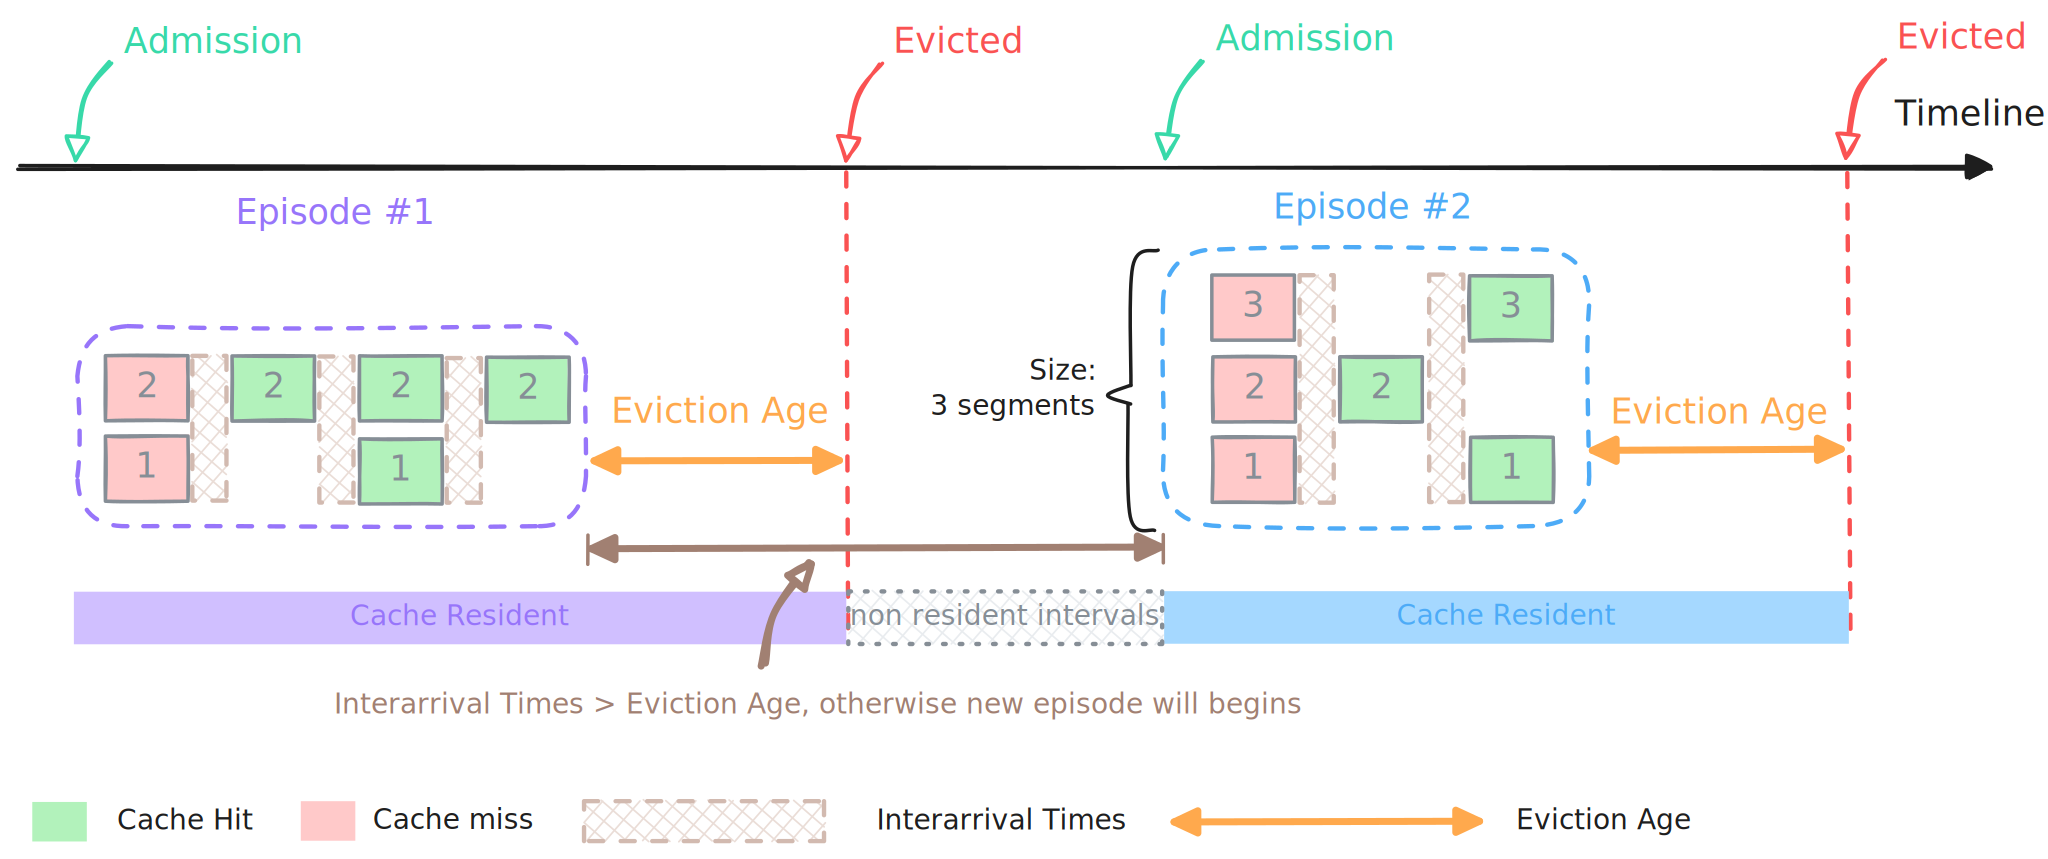
\includegraphics[width=0.5\textwidth]{a9_diagrams/CSCI6806_episode_model.png}
  \caption{Timeline Diagram for Episode Model}
  \label{fig:3}
\end{figure}

Within an episode, all requests that occur during this period are grouped. Writing an object into flash always consumes a fixed flash write cost as long as the object remains in the cache, no matter how many times the object is accessed subsequently before the object is evicted. The benefit of the episodes model is that by treating the entire cache residency as one unit, it reflects the cost of an admission more accurately than the traditional hit rate approach. In addition to the episodes model, the paper introduces an Optimal Admission Policy (OPT). OPT actively selects the episodes that minimizes Peak DT under the constraint of a fixed flash writes budget. However, since the OPT is offline therefore it is not deployable in practice. Instead, the authors use OPT to train the ML admission model to imitate OPT's admission decisions to provide the optimal reduction in backend workload. The authors' approach of using ML-guided admission policy resonates with other scholarly works in the same subject. Yan\& Li design RL-Bélády \cite{yan2020rlbelady}, a caching algorithm that administers admission policies based on improving hit rates. However, the episodes model introduced by the authors here is superior to Yan\& Li's framework because the episodes model reflects the true cost of ownership more accurately than the framework proposed by Yan and Li. Moreover, in this article, Wong and his coauthors explicitly targeted the reduction of backend load to stay within the recommended flash endurance limits. 

\subsection{ML-Guided Admission Policy}

Baleen trains an ML-based admission policy that learns to mimic the decisions of OPT. The model relies on attributes derived from storage traces and recency, frequency proxies, object size, and proximity cues. Both temporal locality and structural hints about workload behavior are intended to be captured in these features \cite{yan2020rlbelady}.

\begin{figure}[ht!]
  \centering
  \includesvg[width=0.50\textwidth]{a1_diagrams/CSCI6806_ML_admission_loop.svg}
  \caption{ML Admission Training Loop. The outer loop aligns the assumed EA with the EA measured in simulation; the inner loop adjusts the admission threshold until the flash write rate reaches the target. Once both converge, EA and the threshold are fixed.}
  \label{fig:4}
\end{figure}

This is an extension of previous ML-based admission systems. For example, Flashield employed lightweight SVM classifiers to admit only "flash-worthy" objects and demonstrated the usefulness of selective admission for endurance \cite{song2020lrb}. The training target of the oracle is the OPT, which sends labels for episodes that should be let in under a flash write constraint. OPT is not implementable online, but it provides a perfect supervision signal. By learning to replicate the OPT's label, Baleen's ML model learns when flash writes are most effective for reducing backend load \cite{yan2020rlbelady}. 

The key goal is to reduce Peak DT, not maximize hit rate. A prior prototype that maximized hit rate alone degraded DT as certain admitted objects added flash writes while doing little to alleviate backend pressure. This indicates why optimizing for hit rate does not coordinate with end-to-end performance of systems \cite{yan2020rlbelady}.

\subsection{ML-Guided Prefetching Policy}

In a bulk storage system, prefetching is applied to minimize DT by requesting additional data that assists in overall low IO operations whenever the data is requested. Prefetching can save backend DT by fetching future segments in advance, but if performed poorly, it costs flash writes and cache space. Thus, Baleen coordinates prefetching with its ML admission policy to ensure prefetching and admission work together effectively.

Baleen models access from the episode, such that aggregate all the accesses for a block of time in which they reside in the cache. From this model, it derives the OPT-Range, which is defined as the minimum set of segments such that all access in an episode will be covered. Baleen's ML-Range model is trained to forecast this minimal segment range, learning the right amount to prefetch without prematurely fetching entire blocks.

It is equally critical to know when to prefetch. Baleen's ML-When evaluates whether the predicted prefetch will indeed bring down this DT more than what it costs in flash writes. Prefetching is activated only if the anticipated benefit is higher than a predetermined confidence threshold.

Through the combination of ML-Range and ML-When with its access policy, Baleen minimizes the number of expensive disk seeks (accesses) without imposing excessive flash wear. In this way, the selective prefetching contributes enormously to decreasing Peak DT and total cost of ownership (TCO).

\subsection{Baleen-TCO}

Baleen-TCO has been designed aiming to minimize the use of system resources with a focus on SSD and HDD write endurance workloads. 

It means, if the SSD is often written, a lower demand for HDD writes will be produced, but at the expense of reducing its lifespan \cite{yang2022cachesack}. On the other hand, if fewer data are written, the life of an SSD will be longer, but there will be strong excessive demand for HDD and a price hike as well \cite{yan2020rlbelady}.
Baleen-TCO includes a controller including an operation to determine the write rate with the smallest write cost. It will derive from HDD cost and SSD cost. It evaluates different flash write rates by measuring the Peak DT and the total flash writes for each option, as shown in Figure~\ref{fig:6}. These values are applied to the TCO function, and the controller selects the write rate that produces the lowest overall cost. Kangaroo also explores cost-aware flash caching by focusing on efficient small-object caching, and its principles of balancing flash endurance with system cost provide context for Baleen-TCO's design.

In Baleen, the TCO metric combines DT reduction, and wear on flash cache, into a single optimization objective. The Baleen approach strikes a fine balance between reduced backend load and flash cache wearouts \cite{mcallister2021kangaroo}.

Total Cost of Ownership (TCO) in this section refers to the combination of the monetary cost of the SSDs as well as the device wear. Here, the assumption is that HDD cost is measured via Peak DT while the cost of SSD is measured via write amplification. 

\clearpage

\section{Related Work}

% one page, no figures

\subsection{Flash caching for HDD-backed bulk storage}

The research in flash caches has the hope of delivering a balanced solution. Overall, the articles explore the question of how to design a caching system that takes care of the issues of performance and endurance. This part of the paper presents an overview of ten years of research in the field and dives into topics such as hybrid storage architectures, adaptive admission, cost modeling, and endurance optimization. These 10 articles together have laid the groundwork for the approach of using the episode model and ML-guided admission and prefetching policies \cite{hsieh2012cachingless, ma2014reliablewriteback, li2015ripq, eisenman2019flashield, berg2020cachelib, mcallister2021kangaroo, xia2021tectonic, wang2023fifo}.

One of the approaches, which focused on bridging the gaps of endurance and performance on HDDs and SSDs, was introduced in \cite{hsieh2012cachingless}. The article explores the possibility of combining HDDs with SSD caches to establish various hybrid storage systems. It concludes that more cache space does not necessarily lead to better performance because SSDs need significant space for garbage collection, so increasing cache space alone undermines endurance and performance. The article proposed the OP-FCL cost model that dynamically adjusts cache size based on the garbage collection overhead in real time. The article first introduced the trade-off between cache size and write amplification that led to the emphasis of later discussions on the TCO. Other related work in this period also focused on partitioning and selective admission. Numerous attempts were made to separate read and write regions in both HDDs and SSDs, and others experimented with new caching methods that used less energy or write buffering -- placing incoming write requests in a temporary buffer (DRAM) before flash to reduce write amplification \cite{ma2014reliablewriteback}.

\subsection{Admission and Prefetching strategies}

ML–provided caching work moved beyond heuristic policies by approximating the Bélády MIN oracle through forecasting models. Learning Relaxed Bélády (LRB) \cite{song2020lrb} introduced a realistic eviction system, relaxing Bélády's hard rule of evicting the furthest-future item, by naming a Bélády boundary, which LRB decides through objects whose next access falls some distance toward the future, and taking Gradient Boosting Machines (GBM) and features of deltas, exponentially decayed counts, and static metadata, respectively, for evicting contender items. Reducing WAN traffic by 4–25\%, compared to production baselines (e.g., B-LRU), and exhibiting modest overhead on real content delivery network servers (CDN), this design reduces WAN traffic and makes CDN infrastructure operations feasible.

Extending this work, RL-Bélády (RLB) \cite{yan2020rlbelady} generalizes the approach to optimizing admission and eviction over an aggregate framework, and blends light-weight next-requirement guessing and reinforcement learning for controllable admission control, and takes Limited Stochastic Optimization (LSO) and Experts Decision Model (EDM) controlling RL instability, respectively. The Figure~\ref{fig:2} shows the architecture of this approach.  Measurements on traces of YouTube, Bilibili, and Iqiyi suggest RLB's superior, higher hit rates and up to 50\%s lower training cost than LRB, and performed especially on relatively steady workloads. Together, these surveys suggest a shift from heuristic, single-point policies toward holistic, ML-advantaged caching frameworks balancing guessing accuracy, controllability, and ease of deployability.

In contrast to Baleen, which adopts an ML-controlled design of jointly managing admission and prefetching trained end-to-end on OPT label predictions given episode-based traces, LRB and RLB seek alternate outlooks. LRB focuses on evacuation, approximating Bélády under a loose-boundary mechanism and Gradient Boosting predictions, and achieves WAN-traffic-reduction substantially in CDN caches at the expense of minimal overhead but no prefetching integration \cite{yan2020rlbelady}. RLB, though more comprehensive than LRB, generalizes learning across admission and evacuation under reinforcement learning and next-request prediction, but again does not achieve end-to-end optimization of Baleen. Relative to the overall TCO and disk-level efficiency of Baleen, LRB, and RLB worry almost exclusively about cache-side hit rates and WAN-traffic-reduction. Therefore, Baleen forms a holistic, system-level ML design, while LRB and RLB emphasize deployable, modular solutions at the expense of decreased complexity and limited optimization range \cite{yan2020rlbelady}.

\subsection{Endurance/Cost-aware flash caches (TCO)}

The architecture of endurance- and cost-aware flash caching usually involves a cluster of SSDs as high performance flash cache acted as buffer for slower but long endurance HDDs with controller utilize heuristic or ML-based feedback mechanism to adjust read/write rate in real time. Based on this perspective, CacheSack is a cache admission optimization algorithm developed by Google, built to reduce the overall TCO of Colossus Flash Cache, the general-purpose flash cache service in Google datacenters \cite{yang2022cachesack}.

Classical static admission policies, for example, Lazy Adaptive Replacement Cache (LARC), required hand-tuned parameters, which in turn meant undesirable flash writes or degraded cache hit ratios. CacheSack addresses these problems by categorizing the cache traffic, modeling disk read/write cost at every level of category, and formulating a knapsack problem in order to derive the admission policies optimally.

It requires four interlinked policies -- AdmitOnWrite, AdmitOnMiss, AdmitOnSecondMiss (LARC), and NeverAdmit -- on different aggressiveness levels. It evades NP-hardness, thus inheriting from combinatorial features of the knapsack problem by adopting an approximation method through the use of the fractional knapsack solved through a greedy algorithm. It emulates the least-recently-used (LRU) policy through a time-to-live (TTL) model and applies ghost caches, buffer cache simulators, and similarity enhancement.

CacheSack was rolled out globally to Colossus Flash Cache in May 2021 and switched on as the default admission algorithm. It's a decentralized, lightweight implementation, not requiring end-user configuration, reducing the cost of adoption. Experimental results from both production and simulation confirm unmistakable gains: 6.5\% lower TCO, 6\% lower disk read, and 26\% lower traffic measured in terms of bytes written to flash compared to LARC \cite{yang2022cachesack}. AdmitOnMiss resulted in the larger hit ratios, but CacheSack provided cheaper cache handling by taking read and write cost into account. CacheSack, in short, is a production-proven system based on theoretical modeling and a lean, distributed design, and is capable of handling large-scale flash cache in the optimal fashion to keep cost minimal and life alive.

\clearpage

\section{Methodology}

% one page, no figures, at least 2 tables

\subsection{Artifact \& Environment Setup}

Following the official Baleen-FAST24 GitHub README for test environment setup, trace data will be downloaded, specifically focusing on "Getting Started" instructions. The main purpose of the artifact repository is to reproduce the simulator results from the Baleen paper published at USENIX FAST 2024 \cite{wong2024baleen}. The repository contains Python code to reproduce the simulator results, with the main instructions located in the README.md, which provides guidance for installation via Conda/pip, trace data download procedures, and step-by-step reproduction commands. The artifact includes preconfigured experiments in the runs/ directory, trace data download script in the data/ directory, analysis notebooks in the notebooks/ directory, and ML models in the tmp/ directory, with the cache simulator code residing in the BCacheSim/ directory. The Table~\ref{tb:repo_analysis_table_1} shows the repository components.

\begin{table}[H]
\centering
\caption{Examination of Baleen-FAST24 repository}
\label{tb:repo_analysis_table_1}
\small
\begin{tabular}[t]{lp{5.8cm}}
\toprule
\textbf{Repository} & https://github.com/wonglkd/Baleen-FAST24 \\
\midrule
\textbf{Commit ID} & 4e3a920 \\
\midrule
\textbf{Notebooks} & \makecell[l]{notebooks/example/example.ipynb \\ notebooks/reproduce/commands.ipynb}\\
\midrule
\textbf{Directory} & \makecell[l]{BCacheSim/ (simulator source code) \\ scripts/ (scripts for figure generation) \\ data/tectonic/201910/Region1/*.trace (traces) \\ runs/example/* (simulation results)} \\
\bottomrule
\end{tabular}
\end{table}

\begin{table}[H]
\centering
\caption{Configuration/Matrics}
\label{tb:analysis_table_1}
\small
\begin{tabular}[t]{lp{5.8cm}}
\toprule
\textbf{Admission Policy} & Admit-All \\
\midrule
\textbf{Prefetch} & Disabled \\
\midrule
\textbf{Eviction Policy} & LRU/DT-SLRU/EDE \\
\midrule
\textbf{Cache size} & 366.475 GB\\
\midrule
\textbf{Trace slices} & data/tectonic/201910/Region1/full\_0\_0.1.trace \\
\bottomrule
\end{tabular}
\end{table}

\subsection{Repository Scope \& Terminology}

The scope of the artifact encompasses the Python simulator code and notebooks for paper-style reproduction of Baleen's ML admission and prefetching policies, while explicitly excluding the unreleased testbed components that modified proprietary CacheLib internals \cite{wong2024baleen}. The terminology mapping reveals that Service Time in the code corresponds to DT in the paper, representing the time spent accessing backend storage, while Chunks in the code are referred to as Segments in the paper, defining the granularity of data management units. Episodes serve as temporal segments used for ML training and analysis, representing coherent periods of cache behavior, with OPT functioning as the baseline for comparison, and DT representing the dependencies between service time measurements and decision thresholds. The key components include BCacheSim as the Python cache simulator specialized for flash caching in bulk storage systems, EpisodicAnalysis as the ML training framework for admission and prefetching models based on episodes, admission policies comprising Baleen (ML-based), RejectX (baseline), and CoinFlip (baseline), eviction policies including LRU and FIFO, and prefetching capabilities with ML-based prefetching featuring configurable ranges such as episode and access-time-episode-predict.

\subsection{Metric Definitions}
A clear set of metrics needs to be defined to evaluate the Baleen article against other heuristic approaches.
 
\subsubsection{DT and Peak DT}
DT is the most straightforward metric to measure the back-end load and refers to the total amount of time the HDD disk heads are active; this metric combines the search time and the time to read an additional byte \cite{wong2024baleen}. Peak DT can be conceptualized as the maximum DT observed in a given timeframe and is more critical than average DT because it reflects the maximum throughput that data storage facilities need \cite{wong2024baleen}. These two metrics will be measured against HDD capacity.

\subsubsection{Flash Write Rate}
Since an SSD has an endurance limit, it imposes restrictions on the usage of flash cache\cite{wong2024baleen,mcallister2021kangaroo}. The total flash write rates will be measured under each admission policy against the rejection threshold. The purpose is to understand how limited flash write rates can be used efficiently to reduce back-end load.

\subsubsection{Estimated TCO}
The TCO will be calculated as the sum of the cost of HDD capacity (driven by Peak DT) and SSD wearout (as a result of flash write rate) \cite{wong2024baleen}. Further, the TCO will be treated not as a static value but as a curve that varies during the course of the experiment. It factors in both flash cache's endurance cost as well as the benefit of reduced backend workload.

\subsubsection{Cache Hit Rate}
Cache Hit Rate can be defined as the number of I/O requests served by the flash cache rather than the HDD backend.  The paper concludes that optimizing the cache hit rate cannot reliably reduce the pressure of the backend \cite{wong2024baleen, yan2020rlbelady}. Therefore, it will be included in the experiment only as a comparative metric against the other metrics.

\subsection{Analysis \& Reporting Plan}

The analysis will aggregate results across evaluation windows using medians and interquartile ranges (IQR), providing a summary of performance that reduces sensitivity to outliers. If resources allow, multiple random seeds will be used, and confidence intervals will be reported to strengthen the statistical reliability of the findings.

Comparisons will focus on baseline admission heuristics and the Baleen policies trained with ML-guided admission and coordinated prefetching \cite{eisenman2019flashield,yang2022cachesack}. The primary emphasis will be on Peak DT, since it reflects backend provisioning requirements, while cache hit rate will appear only as a diagnostic measure.

To explore parameter sensitivity, experiments will sweep the flash write rate constraint as well as the cache size. From these studies, figures are expected to show relationships such as Peak DT as a function of write rate, TCO as a function of write rate, and Peak DT under different cache sizes. These results will help characterize trade-offs between performance, endurance, and cost.

\clearpage

\section{Evaluation}
The Baleen-inspired caching framework evaluation section demonstrates an extensive assessment of its eviction schemes. This section evaluates how the three implemented eviction policies behave under the same workload and how their latency characteristics change with cache size and parameter settings. The evaluation consists of three essential sections which evaluate system performance through policy comparison and cache size impact and parameter influence assessment. The evaluation demonstrates how design choices affect tail latency and hit rate efficiency and policy stability rather than cache size.

\subsection{Comparison of Eviction Policies}
The comparison of the three eviction policies begins with Peak DT, Median DT, and hit-rate measurements under identical conditions. The measurements show both standard and maximum performance levels which demonstrate how policy design affects system reaction time.

\begin{figure}[!ht]
    \centering
    \includegraphics[width=0.45\textwidth]{a4_diagrams/figure1.png}
    \caption{Peak DT across eviction schemes (E0–E2).}
    \label{fig:figure1}
\end{figure}

\begin{figure}[!ht]
    \centering
    \includegraphics[width=0.45\textwidth]{a4_diagrams/figure2.png}
    \caption{Median DT across eviction schemes (E0–E2).}
    \label{fig:figure2}
\end{figure}

\begin{figure}[!ht]
    \centering
    \includegraphics[width=0.45\textwidth]{a4_diagrams/figure3.png}
    \caption{Cache Hit Rate across eviction schemes (E0–E2).}
    \label{fig:figure3}
\end{figure}

The Peak DT measurement in Figure ~\ref{fig:figure1} shows the Peak DT of different eviction schemes Episode Deadline Eviction(EDE), Baleen, Baseline and DT-SLRU. The results show that Baleen outperforms all other forms of eviction policies by a wide margin (on average 12\% more than RejectX, the best-performing non-ML baseline) which is explained by Baleen's episode-based approach to caching, it is not evaluated at the individual access but rather a block of episodes. Baleen's eviction policy along with ML-guided  with prefetching strategies which admit only ranges of segments which were predicted to have high or very high hit rate while turning away low probability entries. It can also be observed that Baleen still outperforms all other forms of eviction policies based on Figure ~\ref{fig:figure1} graph. It's DT-optimized admit policy alone offers significant value.

With the help of Median DT which was calculated with real world workloads and is displayed as a typical pattern for several eviction regimes. Unlike Peak DT, which captures rare but crucial latency peaks, median DT reflects the performance typically experienced during normal system operation. As shown in the results Baleen, RejectX, and Baseline all achieve very similar median DTs around 2.9-3.0 ms, while DT-SLRU and EDE show slightly higher medians at about 3.7 ms each. The relatively flat trend shown by the first three schemes suggests that optimizing for median DT is less sensitive to caching decisions than optimizing for peak load measures. Therefore, caching policy doesn't play a major role in lowering average-case, latency, and performance gains from ML-guided caching only occur when the system has a heavy load, particularly in reducing tail latencies, as Figure~\ref{fig:figure1} demonstrates by comparison with Figure~\ref{fig:figure2}.

The higher median ST in DT-SLRU and EDE traces to inefficient caching behavior under even light loads. DT-SLRU tends to hang on blocks that have been accessed recently but may not be needed again soon. This leads to a waste of cache resources and increases median DT through more frequent cache misses. Likewise, EDE tries to use its history of evictions to predict an object's usefulness for future evictions. However, without the information derived from DT on which Baleen's offline training and real-time evaluation are based, EDE's decisions might not match characteristics in the backend straight away, so service performance goes downhill on a general level, indicated by its longer DT compared to other policies in the experiment.

In Figure~\ref{fig:figure3} different cache eviction policies are compared. Baleen is clearly to be preferred, yielding a hit rate of roughly 9.3\%. Next comes Baseline and RejectX, both at around 7.5\%. While the hit rates of DT-SLRU and EDE fall below 3\%, leaving them far behind. Baleen's dominance in performance owes much to its ML-driven policy for object entry and exit, which bases its decisions on historical access patterns learned from empirical traces. The predictive capability of Baleen's solution allows it to hold on to items that appear likely more frequently in the near future, and so maximizes cache space to fit jobs in hand. Therefore, cache retention efficiency is high and with hit rates higher still. Among the five eviction policies for the experiments, DT-SLRU and EDE are the poorest in terms of hit rates. In the experiment, the DT-SLRU eviction policy often eject items with potential for further reuse prematurely. EDE aims to reduce write amplification by postponing eviction, yet in the process, it accumulates the cache space quickly. This strategy sacrifices hit rate for preserving SSD endurance. Thus, EDE is also less ideal compared to Baleen's approach.
%no bullet point 
%no subsubsection
%========START figure4 from A4 =============================================
\subsection{Cache Size Sensitivity}
The evaluation of Peak DT against different cache sizes from 100 GB to more than 500 GB in Figure~\ref{fig:figure4a} helps determine how eviction strategies perform under various cache capacities. The Baseline LRU policy in Figure~\ref{fig:figure4b} shows a steady and continuous pattern of improvement because Peak DT values decrease from 7.0 ms at small cache sizes to 6.6 ms at larger cache sizes. The working set retention improves when cache size increases because it reduces the need for disk access. The performance improvement from cache expansion becomes less significant when the cache size exceeds 300–400 GB because most essential data remain stored in the cache.

%The performance of DT-SLRU follows a distinct pattern from other policies. As we can see in Figure~\ref{fig:figure4c}, the Peak DT values under DT-SLRU show minimal change from 100 GB to 384 GB cache sizes because most latency overhead comes from internal promotion and demotion operations instead of insufficient storage capacity. The two-list structure of DT-SLRU which includes probation and protected lists generates internal data movement that leads to increased latency. The internal data movements in the system produce higher latency than the actual disk access operations. The policy achieves performance stability when cache size reaches 400 GB because the expanded space reduces the number of list state changes.



\begin{figure}[H]
    \centering
    \subfloat[Peak DT versus cache size for the DT-SLRU policy.]{%
        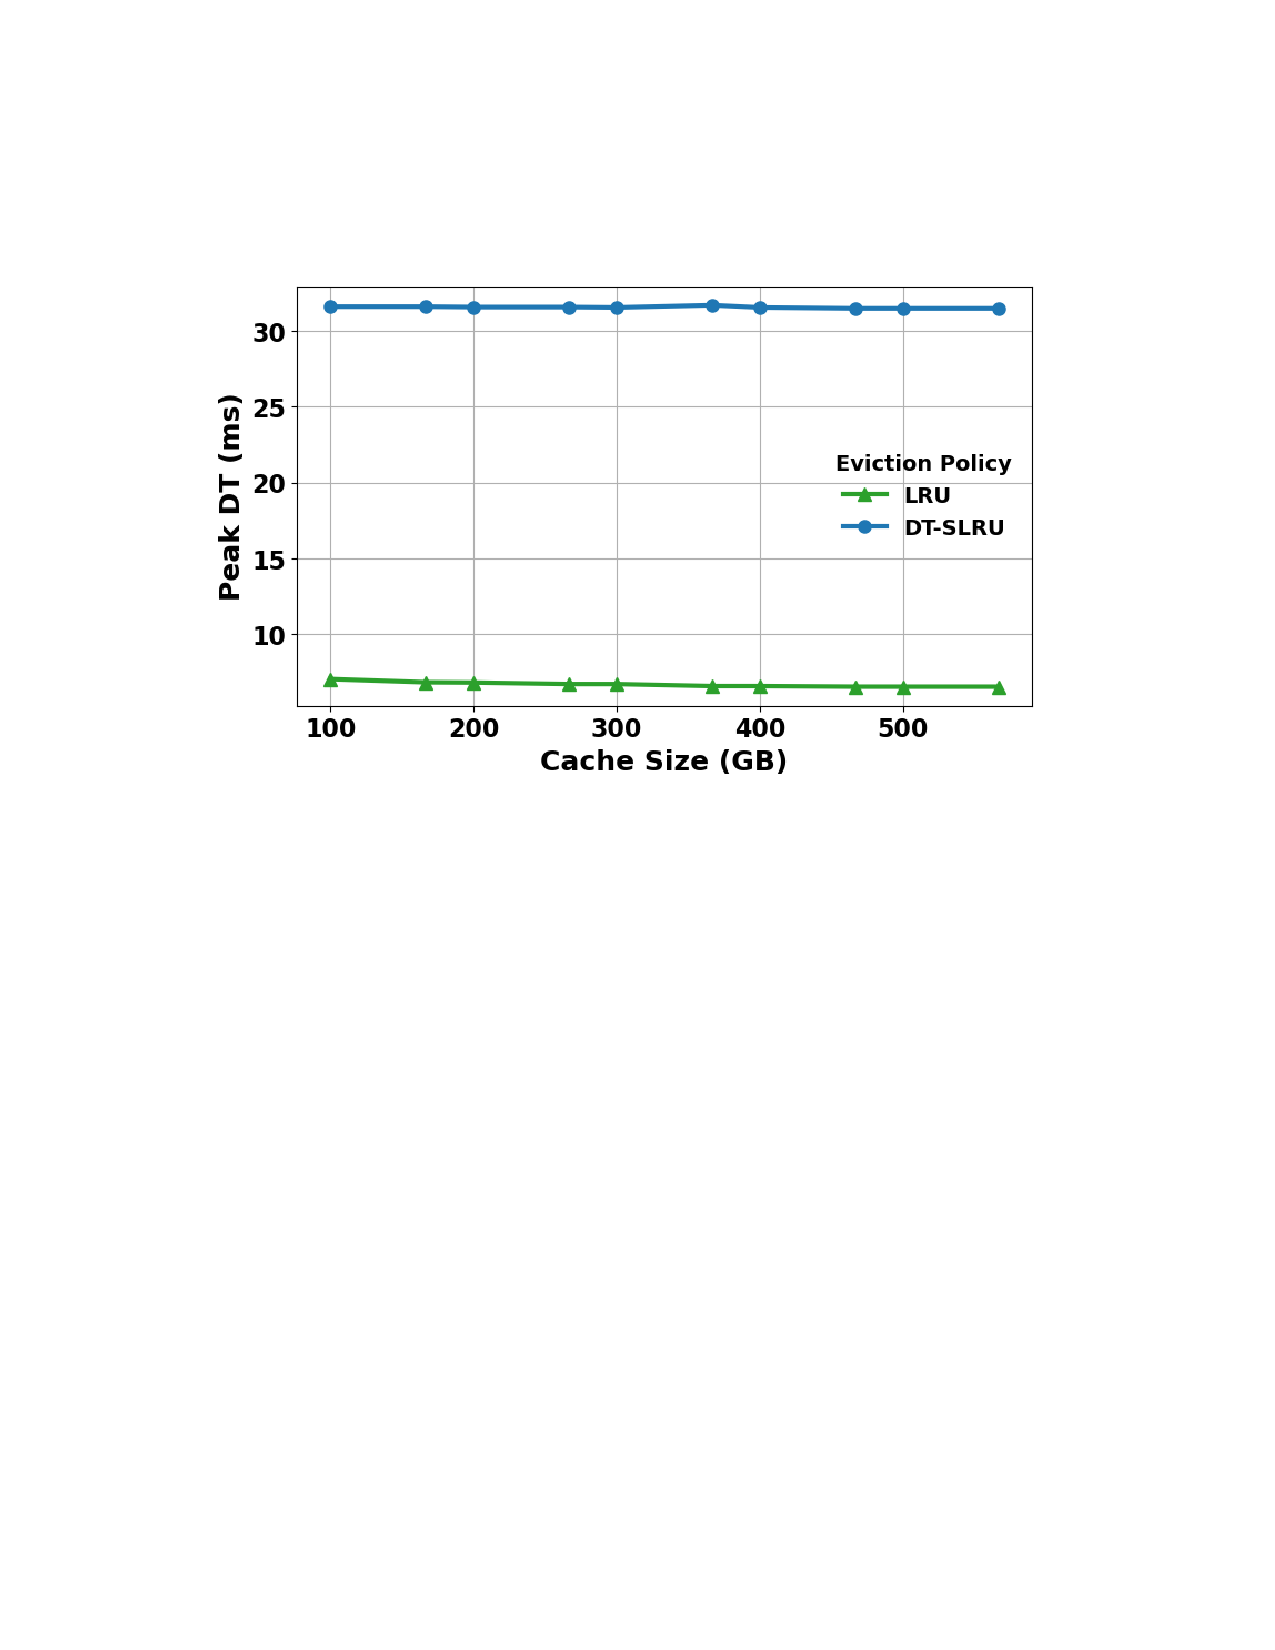
\includegraphics[width=0.48\columnwidth]{a4_diagrams/figure4a.pdf}%
        \label{fig:figure4a}%
    }
    \hfill
    \subfloat[Peak DT variation with cache size under the LRU baseline.]{%
        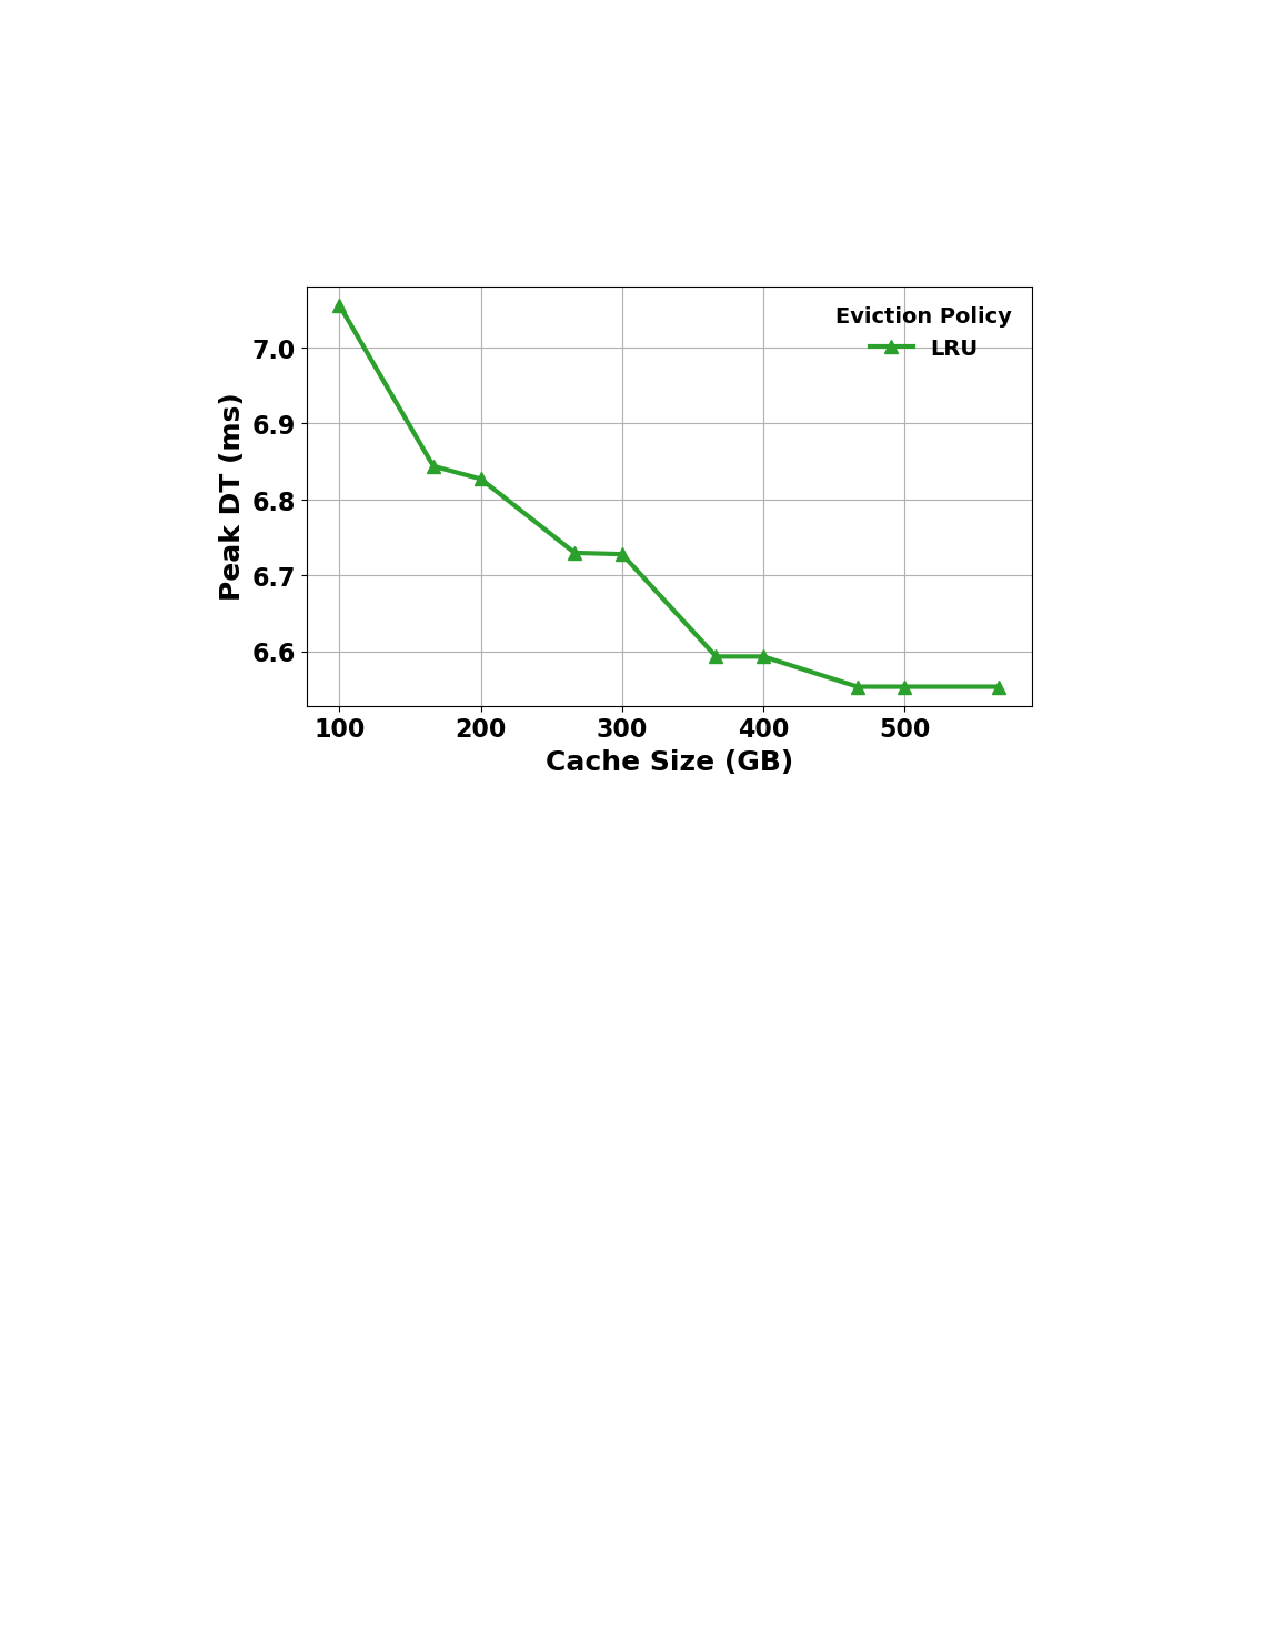
\includegraphics[width=0.48\columnwidth]{a4_diagrams/figure4b.pdf}%
        \label{fig:figure4b}%
    }
    \caption{Peak DT versus cache size for DT-SLRU and LRU policies.}
    \label{fig:peakdt-cache}
\end{figure}

The performance of DT-SLRU shows a distinct pattern from other eviction policies according to Figure~\ref{fig:figure4c} which demonstrates this behavior across different cache sizes. The Peak DT values show minimal variation between 100 GB and 300 GB cache sizes. The main factor that causes latency in DT-SLRU does not stem from insufficient cache space because the system experiences delays from its internal block management operations between probation and protected lists. The process of block promotions and demotions through additional computational operations and metadata updates results in accumulated latency costs that surpass disk operation expenses. The Peak DT values do not decrease substantially when cache size increases below 384 GB.

The Peak DT value experiences a major increase when the cache reaches approximately 384 GB. The particular block distribution and internal thresholds of DT-SLRU create performance issues with this workload when the cache reaches 384 GB. The system requires additional internal block movements during this period which leads to higher Peak DT values. The Peak DT value starts to decrease dramatically when the cache reaches 400 GB. The system achieves stability when the cache reaches 400 GB because it can minimize list transitions. The policy achieves better performance when it has enough space to store frequently accessed data without performing excessive block movements between its internal lists. The system performance of DT-SLRU improves better through minimizing internal block movements instead of depending on cache size expansion.

\begin{figure}[!ht]
    \centering
    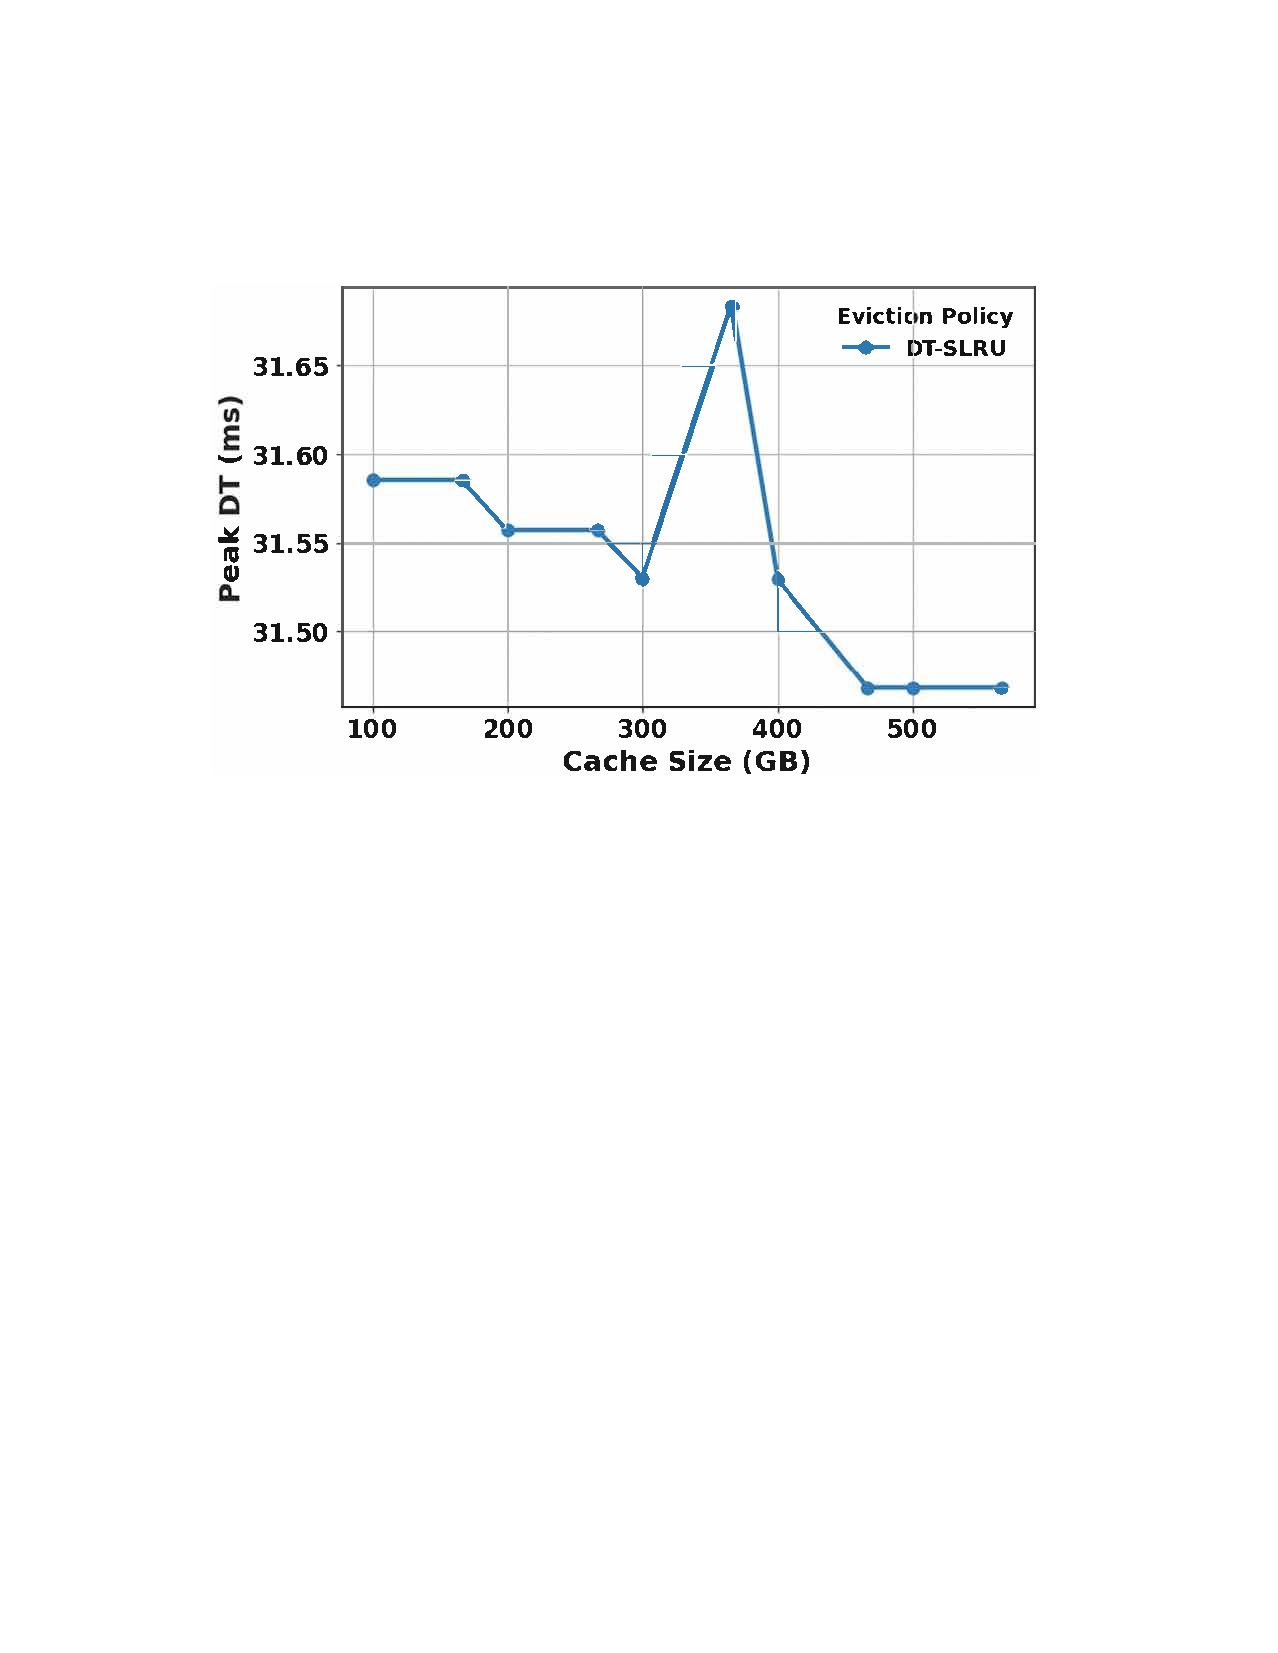
\includegraphics[width=0.50\textwidth]{a4_diagrams/figure4c.pdf}
    \caption{Peak DT versus cache size for the DT-SLRU policy.}
    \label{fig:figure4c}
\end{figure}

The evaluation in Figure~\ref{fig:figure4d} demonstrates that Peak DT depends on eviction logic rather than cache size when all policies operate at the same memory capacity. The policies demonstrate different latency performance levels even though they possess equal memory resources. The highest Peak DT values occur in DT-SLRU because its structural rules produce increased latency when workload patterns mismatch its predefined assumptions. The results show that cache expansion fails to fix performance issues that stem from poor eviction logic design. A policy with poor configuration will maintain its slow performance regardless of the cache size.

%\begin{figure}[t]
%    \centering
%    \subfloat[Peak DT versus cache size for the DT-SLRU policy.]{%
%        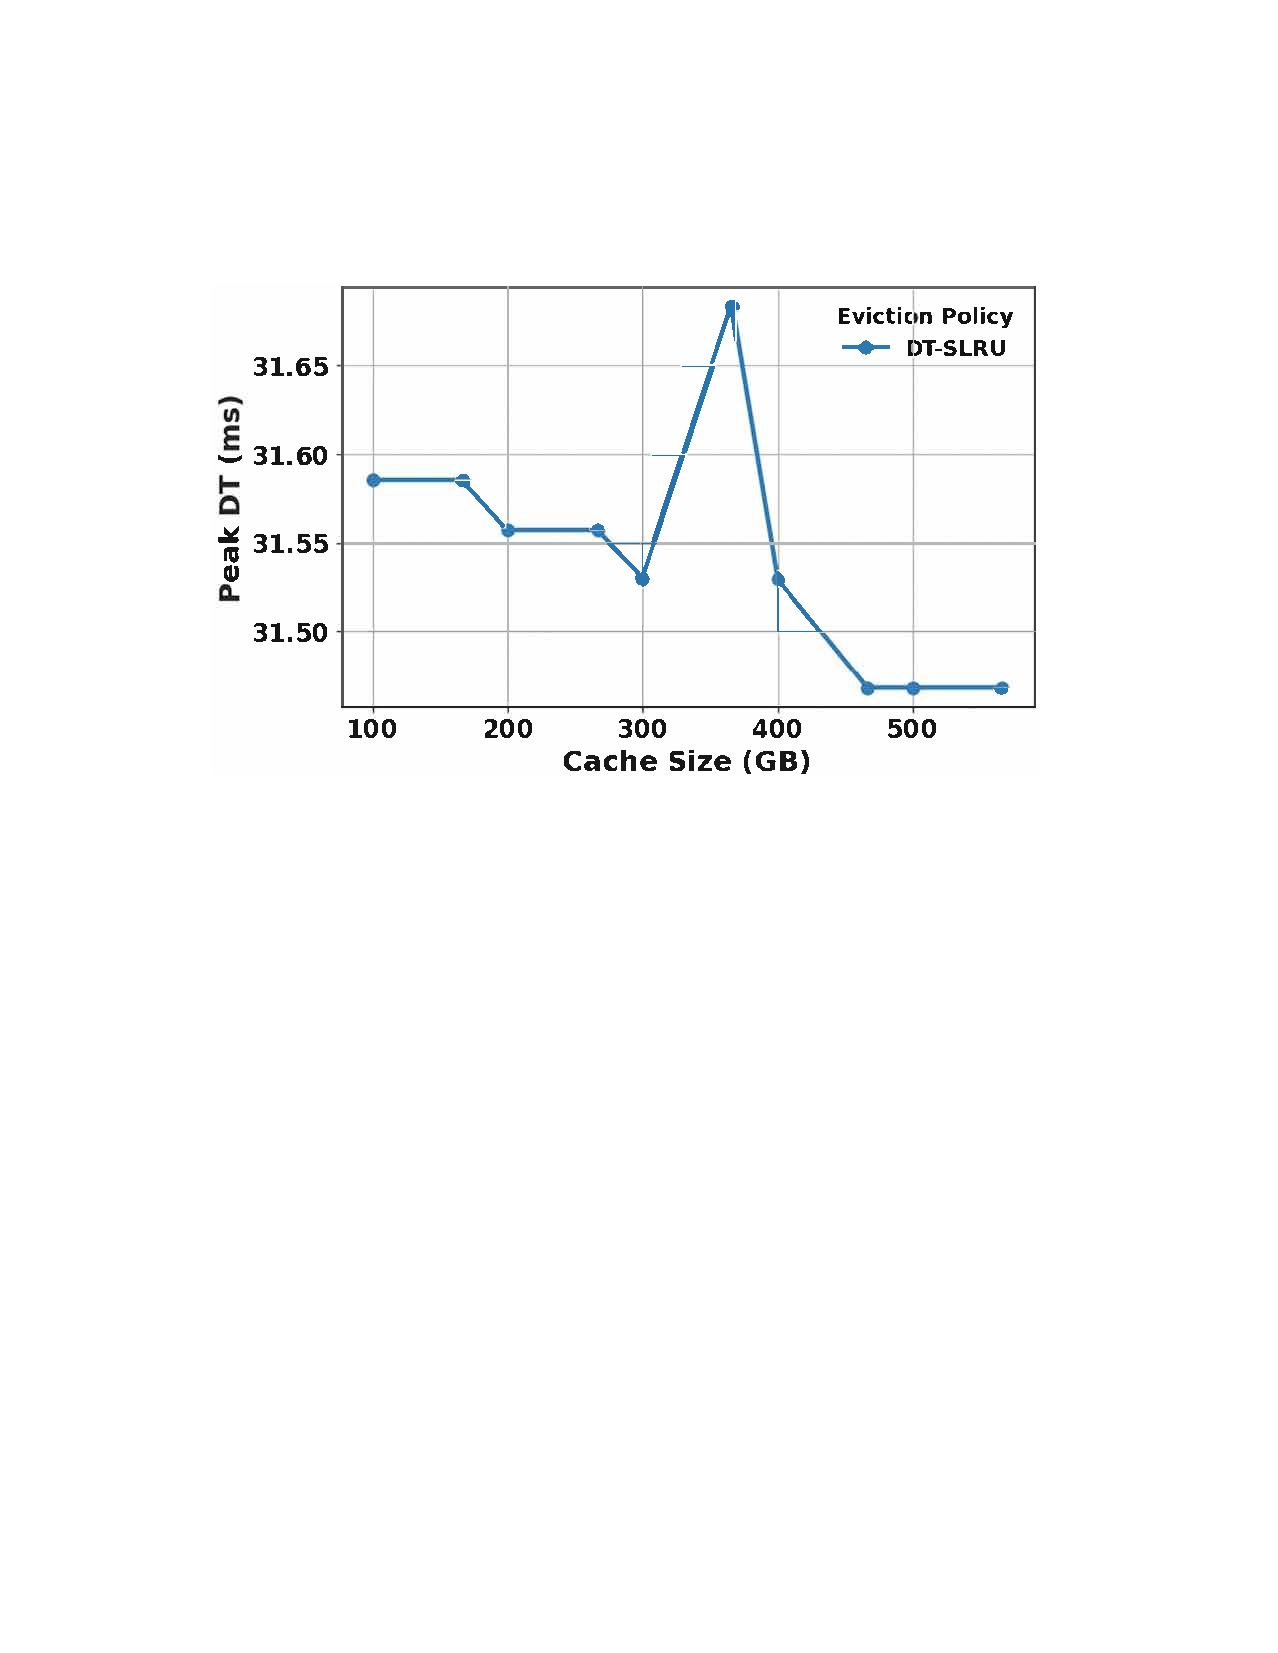
\includegraphics[width=0.48\linewidth]{a4_diagrams/figure4c.pdf}
%        \label{fig:C}
%    }
%    \hfill
%    \subfloat[Comparison of Peak DT across all eviction
%schemes.]{%
%        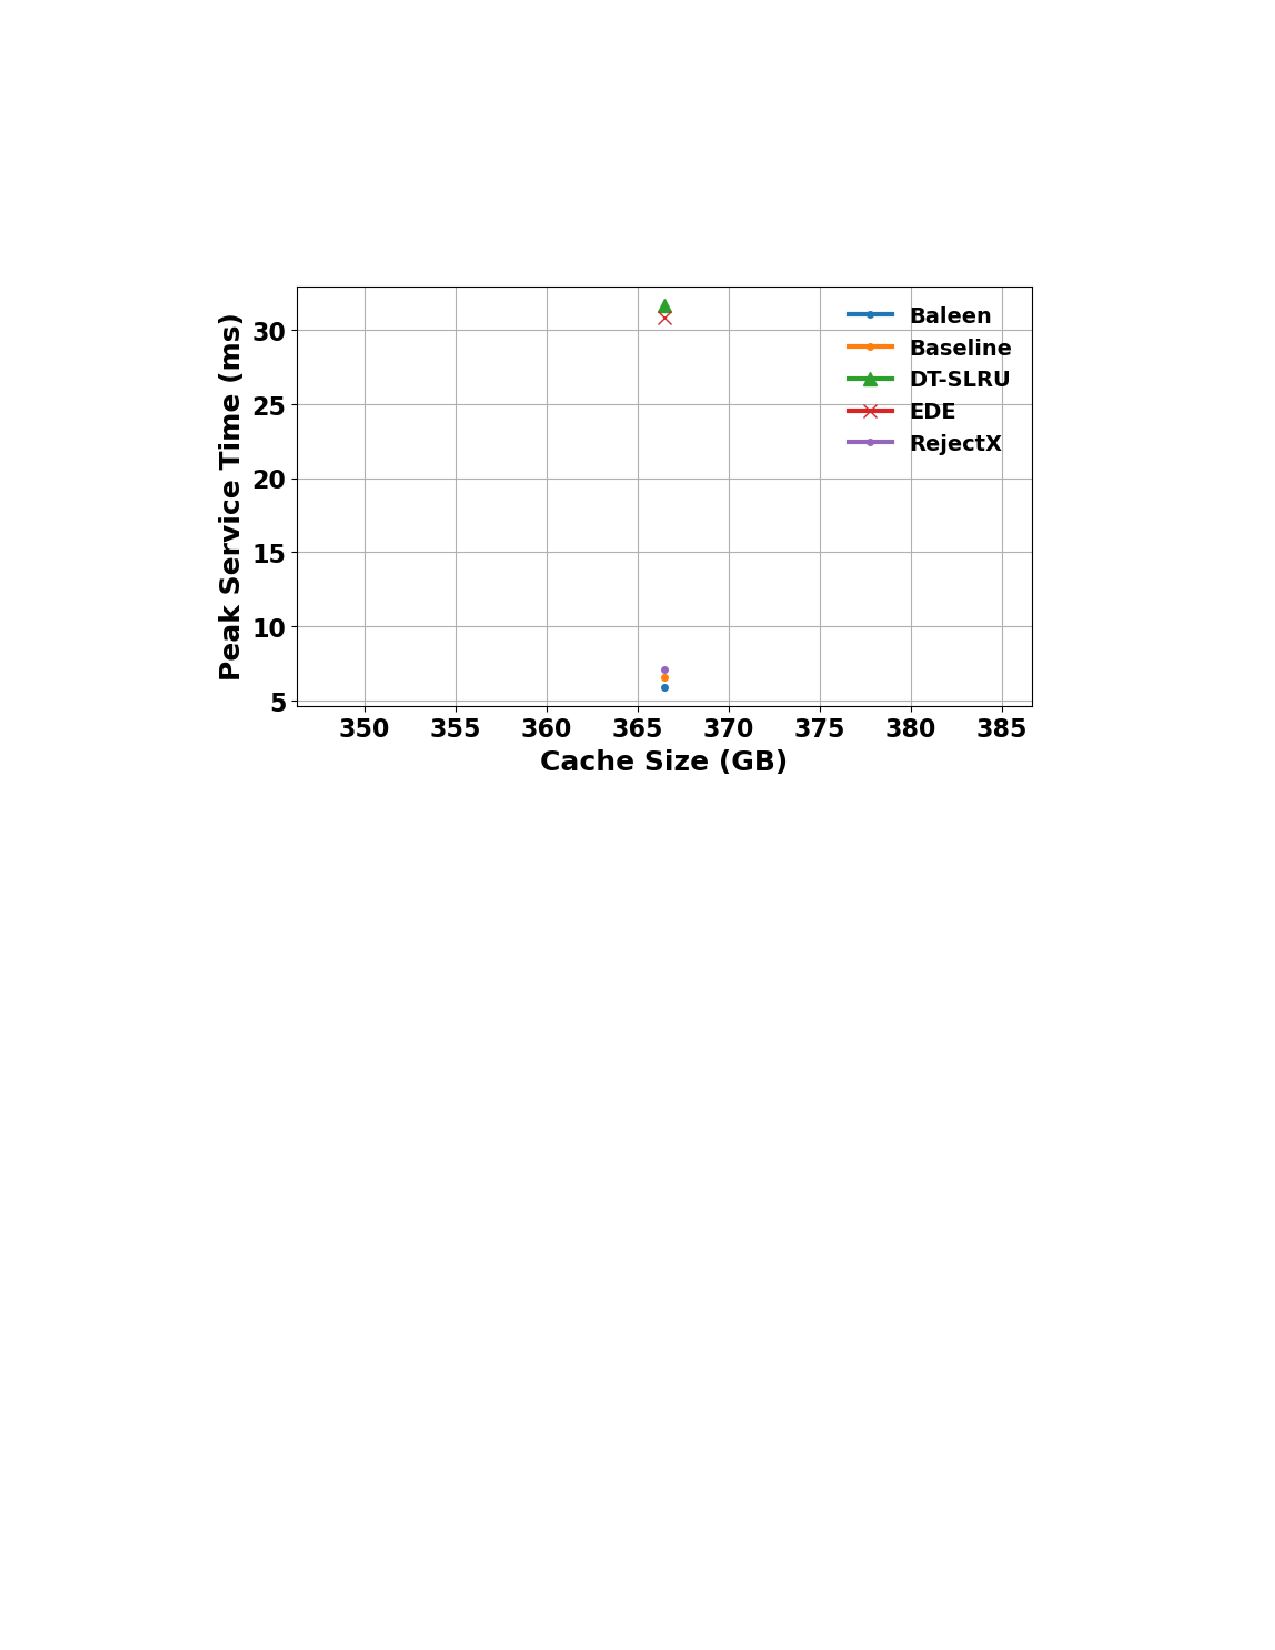
\includegraphics[width=0.48\linewidth]{a4_diagrams/figure4d.pdf}
%        \label{fig:D}
%    }
%    \caption{: caption for all graph}
%    \label{fig:combined}
%\end{figure}
\begin{figure}[!ht]
    \centering
    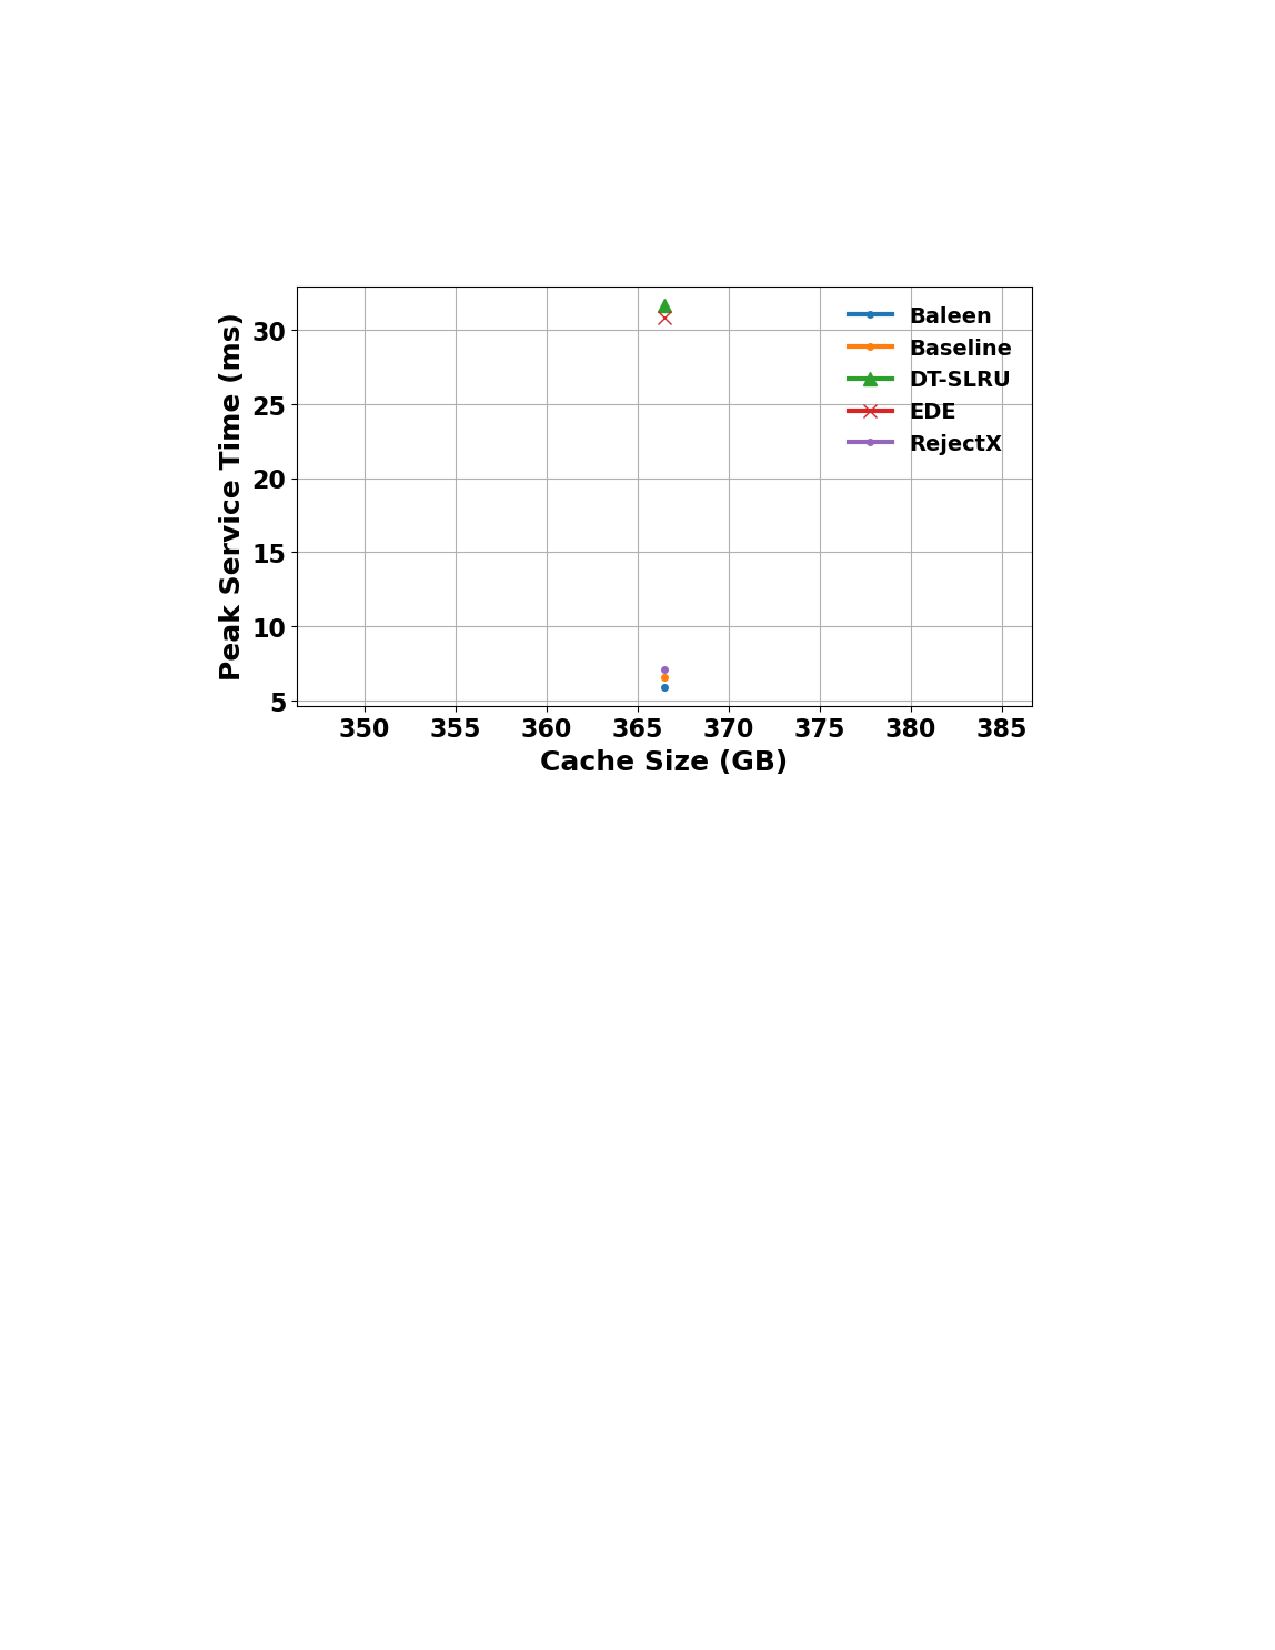
\includegraphics[width=0.50\textwidth]{a4_diagrams/figure4d.pdf}
    \caption{Comparison of Peak DT across all eviction
schemes.}
    \label{fig:figure4d}
\end{figure}
%========END figure4 from A4 =============================================
%========START figure5=========================
\subsection{Sensitivity and Ablation Studies}
The evaluation determine how different control parameter values impact system performance. The evaluation includes two sensitivity analysis sections which test DT-SLRU through $\tau_{DT}$ threshold adjustments and EDE through PROTECTED Cap and $\alpha_{tti}$ parameter modifications

The Peak DT values in Figure~\ref{fig:figure5} demonstrate how the $\tau_{DT}$ parameter affects the DT-SLRU policy. The $\tau_{DT}$ parameter determines the conditions under which a block will transition from the probation list to the protected list. The system promotes all accessed blocks to the protected list at very low $\tau_{DT}$ values which results in intense list transitions. The system experiences increased metadata updates and internal reorganization activities because of excessive state changes which leads to higher Peak DT measurements at minimum $\tau_{DT}$ values. The policy starts to choose blocks for promotion based on increasing $\tau_{DT}$ values. The Peak DT values decrease dramatically when the system transitions between states from 0.002 to 0.004. The curve shows a flat pattern after this point until it reaches its lowest and most stable latency values between 0.006 and 0.016. The policy achieves an optimal balance between system responsiveness and stability when $\tau_{DT}$ values exceed this point. The system becomes unstable because of continuous list transitions when $\tau_{DT}$ values are too low but large thresholds lead to delayed block promotion. The workload achieves its most dependable performance when the $\tau_{DT}$ value falls within the plateau area.
\begin{figure}[!ht]
    \centering
    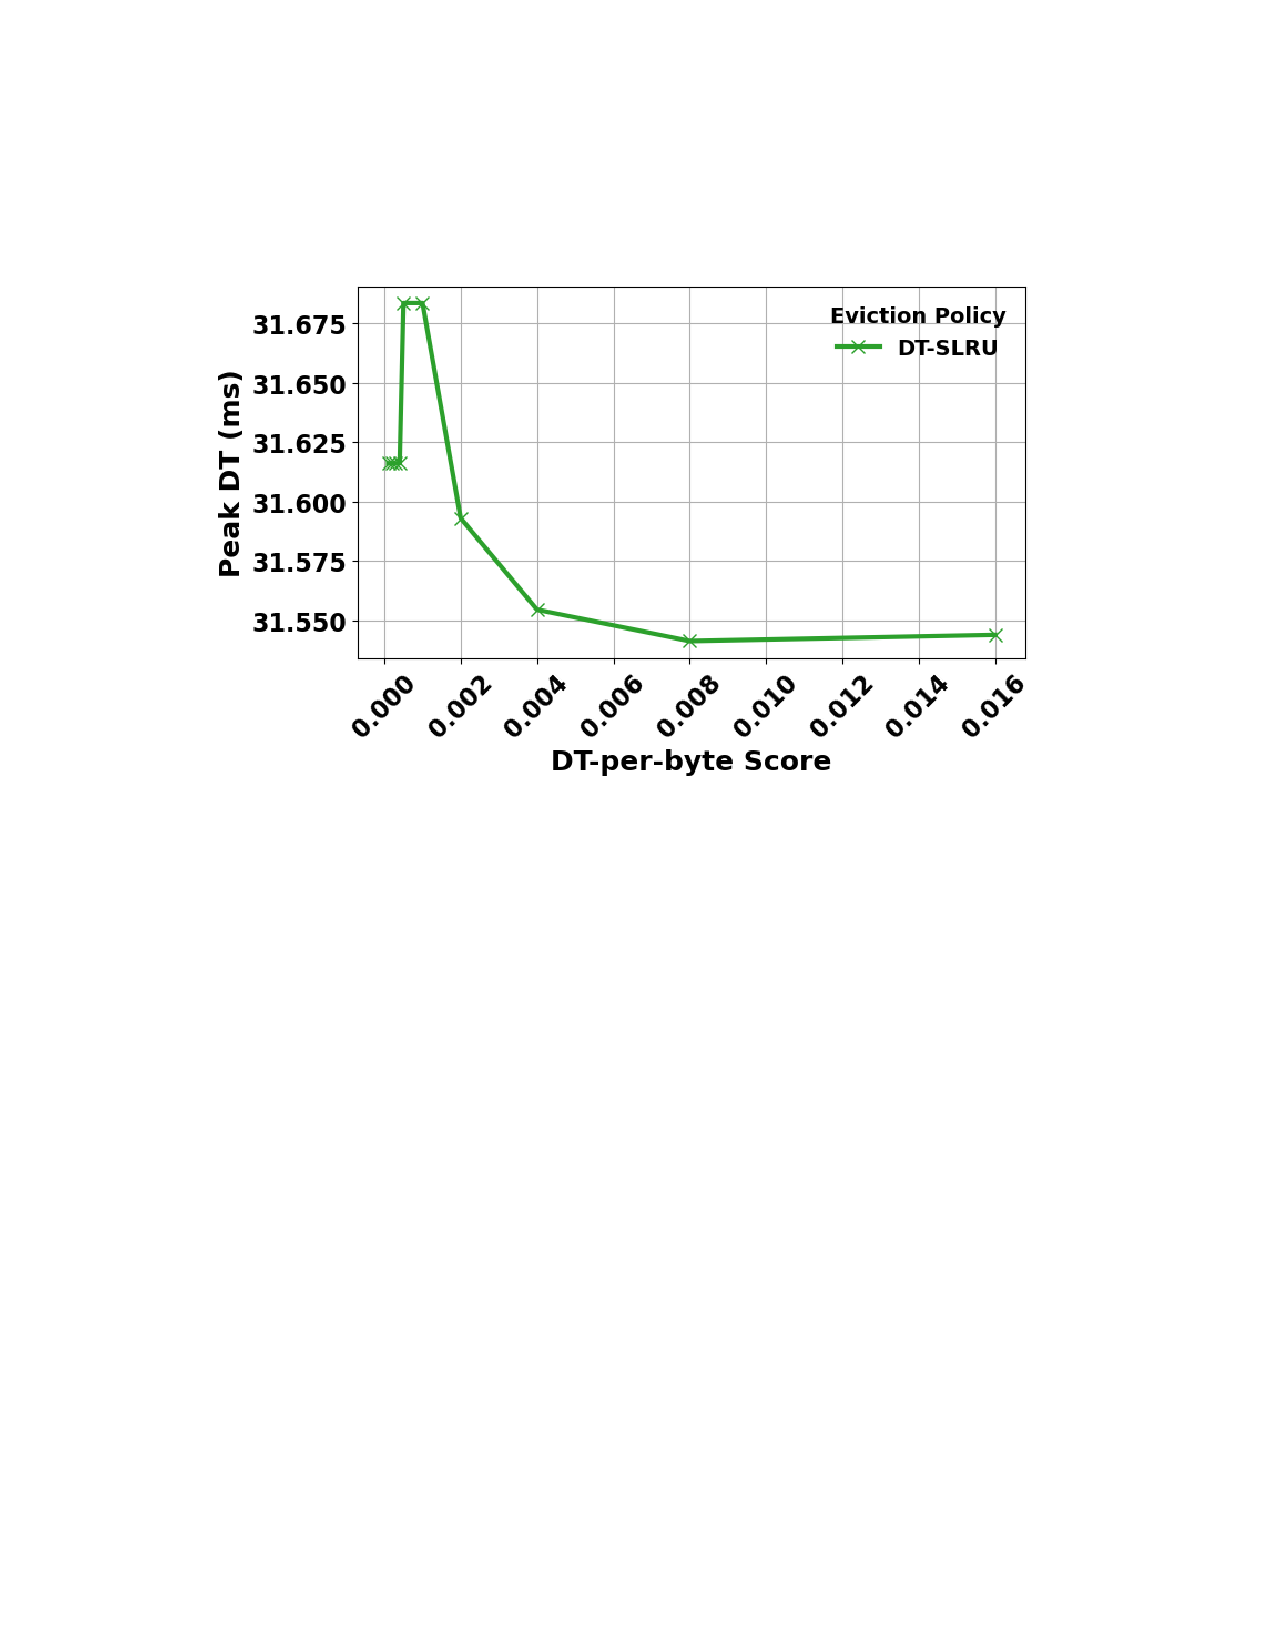
\includegraphics[width=0.50\textwidth]{a4_diagrams/figure5.pdf}
    \caption{Peak DT vs.\ $\tau_{\text{DT}}$ DT-SLRU.}
    \label{fig:figure5}
\end{figure}
%\begin{figure}[!ht]
%    \centering
%    \includegraphics[width=0.50\textwidth]{a4_diagrams/figure6.png}
%    \caption{: Peak DT vs. Protected Cap (EDE).}
%    \label{fig:figure6}
%\end{figure}
\begin{figure}[!ht]
    \centering
    \includegraphics[width=0.50\textwidth]{a4_diagrams/figure7.png}
    \caption{Peak DT vs. $\alpha_{tti}$ (EDE).}
    \label{fig:figure7}
\end{figure}

%The evaluation in Figure~\ref{fig:figure6} demonstrates how different PROTECTED cap ratios affect Peak DT performance under the EDE policy. The evaluation tested five different cap ratios which included 0.1, 0.3, 0.5, 0.7 and 0.9 to achieve the required 0.2 increment step. The Peak DT measurement shows no variation across different values since it stays at 31 ms. The protected and probationary segments' division does not impact tail latency performance for this workload. The object access intervals match episode deadlines under moderate data-reuse patterns so expanding or reducing the protected area does not impact eviction patterns. The protected cap size affects block turnover rates but these effects cancel out in this specific workload trace. The results match previous A4 findings which showed EDE maintained stable performance throughout all parameter adjustments. The episode-deadline logic of EDE controls eviction decisions more strongly than the protected cap settings. EDE delivers consistent performance results regardless of the cache allocation ratio settings.

The evaluation in Figure~\ref{fig:figure7} investigates Peak DT performance when using different values of the smoothing factor $\alpha_{tti}$. The predictor uses this parameter to combine estimated time-to-idle values with episode deadlines for making block eviction decisions. The predictor makes rapid responses to each access when $\alpha_{tti}$ values range from 0.1 to 0.2 which results in short-term changes in eviction decisions. The service time becomes more variable because of these changes which results in higher Peak DT values as shown in the 0.1 data point. The prediction process becomes more stable when $\alpha_{tti}$ values rise because access spikes get distributed through time. The system achieves better deadline stability through this approach which results in lower Peak DT values. The curve reaches its plateau at 0.5 and higher values of $\alpha_{tti}$ do not produce any significant changes in system behavior. The system achieves an optimal point between its ability to respond quickly and maintain stability.

The system's ability to interpret temporal locality depends directly on the $\alpha_{tti}$ value which produces a stronger impact on latency than the PROTECTED Cap ratio. The system becomes too reactive to short-term noise when using small $\alpha_{tti}$ values but becomes too slow to adapt when the workload shifts to a new phase at high values. The Peak DT measurement shows a narrow range of 30.8–30.9 ms but adjusting $\alpha_{tti}$ values can produce significant improvements in tail-latency stability for applications with bursty traffic patterns. The cache achieves optimal performance when $\alpha_{tti}$ values range between 0.5 and 0.7 because it responds well to phase transitions without creating excessive block movements. The results confirm Baleen's design approach because smoothing improves eviction accuracy by removing brief access patterns. The $\alpha_{tti}$ parameter functions as an operational control which enables users to achieve dependable system performance during changing workload patterns.

The evaluation results show that eviction logic produces greater latency effects than cache size does when operating independently. The performance of LRU improves when the cache size increases but DT-SLRU and EDE need specific internal parameter adjustments to reach their optimal performance. The performance of DT-SLRU improves when list transitions become less frequent and EDE achieves better results through adjustments to its idle-time smoothing factor instead of PROTECTED Cap ratio settings. The results show that system performance improves through reduced unnecessary system operations and parameter selections that match workload characteristics. The policies show improved predictability when configured correctly but incorrect parameter values lead to elevated tail latency. The evaluation of all three eviction schemes under identical workload conditions has been finished to establish their reaction patterns when capacity and configuration settings change. The obtained knowledge helps users pick suitable eviction methods for systems that handle different and unpredictable access patterns.

\clearpage

\section{Discussion}

%The results of this study provide a broader understanding of how Baleen's ML-guided design influences flash-cache behavior and how its internal parameters affect performance under different workloads. The evaluation confirms that Peak DT, rather than median latency or hit rate, is the most meaningful metric for assessing backend pressure and long-term system cost. Across all experiments, Baleen consistently reduced tail latency compared with heuristic baselines, demonstrating that coordinated admission, eviction, and prefetching offer benefits in environments where write endurance and backend saturation are critical constraints. These findings reinforce the idea that caching effectiveness cannot be judged solely by local hit-rate optimizations, but must instead consider global effects on backend load.

%The comparison between eviction schemes highlights a clear separation between approaches that rely on short-term recency information and those that incorporate episode-based or deadline-aware decision making. DT-SLRU and EDE both attempt to include service-time insights, yet their performance remains sensitive to parameter choices and workload characteristics. Their median latencies are comparable to simpler heuristics, but their tail behavior worsens under transitions or when internal promotion logic does not align with access patterns. By contrast, Baleen benefits from offline-trained admission and prefetching models that anticipate multi-access episodes and avoid unnecessary flash writes, enabling it to maintain lower Peak DT even without aggressive parameter tuning. This demonstrates the value of coordinated ML-based policies in stabilizing latency in large-scale storage systems.

%The ablation results extend this interpretation by revealing how individual tuning parameters contribute to system behavior. The DT-SLRU threshold $\tau_{DT}$ shows a sharp and highly non-linear influence on Peak DT, indicating that small misconfigurations can amplify backend pressure. In contrast, the PROTECTED Cap parameter in EDE shows almost no effect for this workload, suggesting that EDE's structural deadline-driven logic dominates its internal partitioning. The smoothing factor $\alpha_{tti}$ affects stability more gradually, increasing resilience to bursty access patterns when its value is moderate but offering diminishing returns beyond a certain range. These observations indicate that heuristic schemes either require careful parameter tuning or remain fixed in behavior regardless of configuration. Baleen's ML-guided admission and prefetching avoid these extremes by adapting to long-term access structure rather than relying on static thresholds.

%Although the simulation results demonstrate consistent patterns, several limitations must be acknowledged when interpreting the findings. The analysis relies on a controlled simulator with fixed seek times, constant disk behavior, and a single large-scale Tectonic workload slice. Real systems may exhibit more complex interactions, such as SSD internal parallelism, queue reordering, or dynamic garbage-collection effects that are not represented in the simulator. The parameter sweeps in the ablation study focused on coarse increments and targeted only isolated components of DT-SLRU and EDE, while prefetching and ML-based admission remained disabled for correctness. Broader studies involving coordinated variations may reveal additional interactions that do not appear in isolated experiments. Despite these limitations, the trends observed across multiple figures suggest that the relationship between parameter design and tail-latency stability is robust.

%Beyond direct performance insights, the results have implications for cache design in modern datacenters. The high sensitivity of $\tau_{DT}$ suggests that threshold-driven eviction policies may be effective only within a narrow configuration range, which is difficult to maintain in dynamic or multi-tenant environments. Conversely, the stability of EDE across most parameters implies that deadline-based heuristics, while easy to deploy, offer limited opportunities for optimization. Baleen's behavior demonstrates the advantage of policies that capture episode-level structure and multi-access correlations, enabling the system to mitigate backend bursts rather than react to them after they occur. This distinction is important in large-scale deployments where workload variability makes static heuristics brittle.

%Another observation is the role of prefetching in amplifying the effect of ML-based admission. While prefetching was disabled during ablation for correctness, the evaluation results suggest that coordinated prefetching enables Baleen to reduce Peak DT not only by optimizing what enters the cache, but also by shaping when request bursts reach the backend. Prefetching aligns internal cache state with predicted future episodes, smoothing out incoming peaks. This interaction between admission and prefetching highlights the importance of holistic design rather than treating each subsystem independently and suggests that evaluating caching systems solely through hit-based metrics may underestimate the benefits of coordinated ML-driven mechanisms.

%A broader consideration emerging from these results concerns deployment stability in shared storage environments. The consistent reduction of Peak DT demonstrated by Baleen suggests that ML-guided caching can act as a stabilizing layer that absorbs short-term workload variability rather than amplifying it, which is often the case for heuristic policies. This behavior indicates that systems relying on learned access-pattern predictions may provide more predictable performance under multi-tenant contention and shifting access distributions. Such stability characteristics are relevant for datacenter operators seeking to minimize backend volatility without continuous manual parameter tuning.

%If the project were extended over the next six months, several directions would offer meaningful opportunities for deeper investigation. A natural next step would be to evaluate multiple workloads, including write-heavy, highly bursty, or multi-tenant traces, to capture a broader range of behaviors and stress patterns. Another direction involves testing Baleen's ML admission and prefetching on real hardware or emulation environments to validate that DT improvements persist under device-level variability. Additional ablation studies could jointly vary admission thresholds, deadline predictors, and prefetching confidence levels to uncover coupled effects between system components. Evaluating long-term SSD endurance and measuring the associated changes in TCO would provide practical insights for datacenter deployment. Finally, studying how Baleen adapts under dynamically shifting workloads, where models may require periodic retraining or online fine-tuning, would extend its applicability to evolving environments. Overall, the evaluation and ablation results presented in this work form a strong foundation for these future explorations by showing how ML-guided designs reshape cache behavior under realistic flash-cache constraints.

The results of this study provide a broader understanding of how Baleen's ML-guided design influences flash-cache behavior and how its internal parameters affect performance under different workloads. The evaluation confirms that Peak DT, rather than median latency or hit rate, is the most meaningful metric for assessing backend pressure and long-term system cost. Across all experiments, Baleen consistently reduced tail latency compared with heuristic baselines, demonstrating that coordinated admission, eviction, and prefetching offer benefits in environments where write endurance and backend saturation are critical constraints. These findings reinforce the idea that caching effectiveness cannot be judged solely by local hit-rate optimizations, but must instead consider global effects on backend load.

The comparison between eviction schemes highlights a clear separation between approaches that rely on short-term recency information and those that incorporate episode-based or deadline-aware decision making. DT-SLRU and EDE both attempt to include service-time insights, yet their performance remains sensitive to parameter choices and workload characteristics. Their median latencies are comparable to simpler heuristics, but their tail behavior worsens under transitions or when internal promotion logic does not align with access patterns. By contrast, Baleen benefits from offline-trained admission and prefetching models that anticipate multi-access episodes and avoid unnecessary flash writes, enabling it to maintain lower Peak DT even without aggressive parameter tuning. This demonstrates the value of coordinated ML-based policies in stabilizing latency in large-scale storage systems.

%The ablation results extend this interpretation by revealing how individual tuning parameters contribute to system behavior. The DT-SLRU threshold τ_DT shows a sharp and highly non-linear influence on Peak DT, indicating that small misconfigurations can amplify backend pressure. In contrast, the PROTECTED Cap parameter in EDE shows almost no effect for this workload, suggesting that EDE's structural deadline-driven logic dominates its internal partitioning. The smoothing factor α_tti affects stability more gradually, increasing resilience to bursty access patterns when its value is moderate but offering diminishing returns beyond a certain range. These observations indicate that heuristic schemes either require careful parameter tuning or remain fixed in behavior regardless of configuration. Baleen's ML-guided admission and prefetching avoid these extremes by adapting to long-term access structure rather than relying on static thresholds.

The ablation results extend this interpretation by revealing how individual tuning parameters contribute to system behavior. The DT-SLRU threshold $\tau_{\text{DT}}$ shows a sharp and highly non-linear influence on Peak DT, indicating that small misconfigurations can amplify backend pressure. In contrast, the PROTECTED Cap parameter in EDE shows almost no effect for this workload, suggesting that EDE's structural deadline-driven logic dominates its internal partitioning. The smoothing factor $\alpha_{\text{tti}}$ affects stability more gradually, increasing resilience to bursty access patterns when its value is moderate but offering diminishing returns beyond a certain range. These observations indicate that heuristic schemes either require careful parameter tuning or remain fixed in behavior regardless of configuration. Baleen's ML-guided admission and prefetching avoid these extremes by adapting to long-term access structure rather than relying on static thresholds.

%======================
The conclusion is clear: DT-Per-Byte Score (DT-SLRU), indeed has a huge impact on Peak DT, demonstrating a basic sensibility in terms of how hard the cache holds on to blocks. For very small DT-Per-Byte (e.g., 0.001), the cache still caches blocks that reduce the service time only a little. These blocks do not experience useful reuse before eviction so Peak DT does not offer improvement and flash writes increase since we maintain unneeded blocks. These blocks exist in flash cache without decreasing the backend load, thus resulting in waste of flash space and larger write amplification

This demonstrates that DT-SLRU is very sensitive to the choice of the DT-Per-Byte Score. Adjusting this parameter becomes particularly important in finding a trade-off between flash endurance and sustained service time benefits.
%===================================


Another observation is the role of prefetching in amplifying the effect of ML-based admission. While prefetching was disabled during ablation for correctness, the evaluation results suggest that coordinated prefetching enables Baleen to reduce Peak DT not only by optimizing what enters the cache, but also by shaping when request bursts reach the backend. Prefetching aligns internal cache state with predicted future episodes, smoothing out incoming peaks. This interaction between admission and prefetching highlights the importance of holistic design rather than treating each subsystem independently and suggests that evaluating caching systems solely through hit-based metrics may underestimate the benefits of coordinated ML-driven mechanisms.

A broader consideration emerging from these results concerns deployment stability in shared storage environments. The consistent reduction of Peak DT demonstrated by Baleen suggests that ML-guided caching can act as a stabilizing layer that absorbs short-term workload variability rather than amplifying it, which is often the case for heuristic policies. This behavior indicates that systems relying on learned access-pattern predictions may provide more predictable performance under multi-tenant contention and shifting access distributions. Such stability characteristics are relevant for datacenter operators seeking to minimize backend volatility without continuous manual parameter tuning.

Although the simulation results demonstrate consistent patterns, several limitations must be acknowledged when interpreting the findings. The analysis relies on a controlled simulator with fixed seek times, constant disk behavior, and a single large-scale Tectonic workload slice. Real systems may exhibit more complex interactions, such as SSD internal parallelism, queue reordering, or dynamic garbage-collection effects that are not represented in the simulator. The parameter sweeps in the ablation study focused on coarse increments and targeted only isolated components of DT-SLRU and EDE, while prefetching and ML-based admission remained disabled for correctness. Broader studies involving coordinated variations may reveal additional interactions that do not appear in isolated experiments. Despite these limitations, the trends observed across multiple figures suggest that the relationship between parameter design and tail-latency stability is robust.

If the project were extended over the next six months, several directions would offer meaningful opportunities for deeper investigation. A natural next step would be to evaluate multiple workloads, including write-heavy, highly bursty, or multi-tenant traces, to capture a broader range of behaviors and stress patterns. Another direction involves testing Baleen's ML admission and prefetching on real hardware or emulation environments to validate that DT improvements persist under device-level variability. Additional ablation studies could jointly vary admission thresholds, deadline predictors, and prefetching confidence levels to uncover coupled effects between system components. Evaluating long-term SSD endurance and measuring the associated changes in TCO would provide practical insights for datacenter deployment. Finally, studying how Baleen adapts under dynamically shifting workloads, where models may require periodic retraining or online fine-tuning, would extend its applicability to evolving environments. Overall, the evaluation and ablation results presented in this work form a strong foundation for these future explorations by showing how ML-guided designs reshape cache behavior under realistic flash-cache constraints.


\clearpage

\section{Ablation Study}

The ablation study varies individual parameters while disabling ML-based admission and prefetching so that only eviction-related mechanisms affect the results. This setup makes it possible to see how DT-SLRU and EDE behave when their internal controls change, and which parameters meaningfully influence tail latency.
\begin{figure}[H]
  \centering
  \includegraphics[width=0.4950\textwidth]{a5_diagrams/A5 figure 1.png}
  \caption{Peak DT vs $\tau_{DT}$ (DT-SLRU). Peak DT rises as only a few blocks are promoted to the protected segment, then declines once the threshold becomes less restrictive.}
  \label{fig:13}
\end{figure}

Figure~\ref{fig:13} shows how Peak DT changes as the $\tau_{DT}$ threshold varies. DT-SLRU is very sensitive to this parameter: very small $\tau_{DT}$ values promote almost every referenced block, causing heavy churn in the protected list and keeping Peak DT high. Increasing $\tau_{DT}$ reduces promotion frequency and quickly lowers Peak DT until the system reaches a stable region. Beyond that point, the effect levels off and additional increases bring little benefit. This makes $\tau_{DT}$ the main tuning knob for DT-SLRU because it directly shapes tail-latency behavior.
\begin{figure}[H]
  \centering
  \includegraphics[width=0.4950\textwidth]{a5_diagrams/A5 figure 2.png}
  \caption{Hit Rate vs $\tau_{DT}$ (DT-SLRU). The hit rate increases as $\tau$DT grows, showing that more frequent promotions help reuse cached data. Then the curve becomes almost flat, meaning that raising $\tau_{DT}$ further brings almost no improvement.}
  \label{fig:14}
\end{figure}

Figure~\ref{fig:14} shows the corresponding hit-rate behavior for the same threshold sweep. Unlike Peak DT, the hit rate changes only slightly across the range. The curve stays mostly flat, with moderate improvement only in the region where Peak DT stabilizes. This means the reduction in Peak DT is mainly the result of lower internal churn rather than a strong increase in reuse. DT-SLRU achieves its most balanced behavior in the middle $\tau_{DT}$ range, where promotions are neither too aggressive nor too restrictive.
\begin{figure}[H]
%\begin{figure}[H]
    \centering
    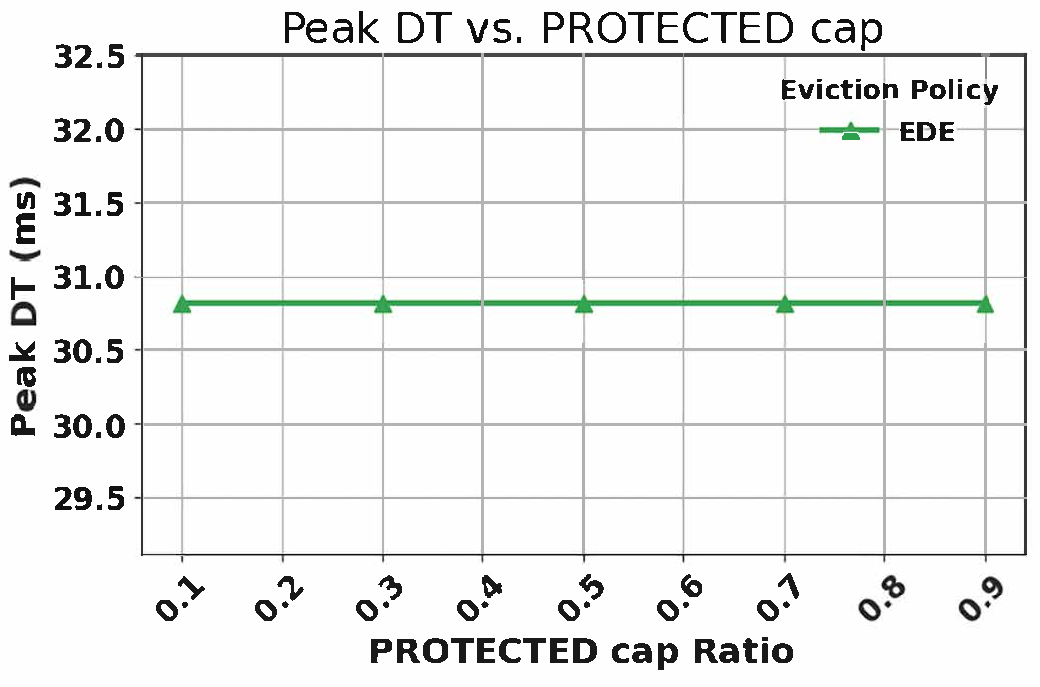
\includegraphics[width=0.4950\textwidth]{a5_diagrams/A5_figure_3.png}
    \caption{Peak DT vs. PROTECTED Cap (EDE). The parameter is varied between 0.1 and 0.9 with an increment of 0.2.}
    \label{fig:15}
\end{figure}

Figure~\ref{fig:15} illustrates the effect of the PROTECTED Cap ratio for EDE. In contrast to DT-SLRU, EDE shows almost no sensitivity to this parameter. Peak DT is nearly identical across all tested values, which suggests that the split between protected and probation segments does not strongly influence EDE's eviction decisions. This aligns with the design of EDE, where eviction deadlines matter more than static segment sizes. For this workload, increasing the protected portion does not significantly alter deadline predictions, so tail-latency behavior remains stable.
\begin{figure}[H]
    \centering
    \includegraphics[width=0.4950\textwidth]{a4_diagrams/figure6.png}
    \caption{Peak DT vs. PROTECTED Cap (EDE) for Evaluation. The parameter is varied between 0.1 and 0.9 with an increment of 0.1.}
    \label{fig:figure6}
\end{figure}

As shown by comparing Figure~\ref{fig:15} and Figure~\ref{fig:figure6}, the PROTECTED Cap curves for EDE in the ablation study and in the evaluation section are nearly identical. Both sweeps use the same parameter range from 0.1 to 0.9, with the only difference being the step size: the evaluation sweep varies the parameter with 0.1 increments, while the ablation sweep follows the required 0.2 spacing. Because EDE's behavior is insensitive to this parameter for this workload, changing the resolution of the sweep does not alter the shape of the curve or its interpretation. The similarity between the two figures confirms that the PROTECTED Cap ratio has little effect on Peak DT and that EDE's eviction decisions are primarily driven by deadline predictions rather than segment allocation.

For a similar reason, the ablation plot for the $\alpha_{tti}$ parameter is not included as a separate figure in this section. The evaluation section already contains an identical plot, shown earlier as Figure~\ref{fig:figure7}, which was generated using the same parameter range and workload configuration that later appeared in the ablation instructions. Because the resulting curve matches the ablation version exactly, reproducing the figure here would duplicate Figure~\ref{fig:figure7} without adding new information. The discussion for $\alpha_{tti}$ in this section therefore refers directly to the previously presented result.

The similarity between the evaluation and ablation sweeps for both parameters further illustrates that EDE's behavior is mostly determined by its deadline predictions rather than by fine-grained tuning. Since the underlying access patterns and estimated deadlines are identical across both experiments, the policy produces nearly the same response even when parameter step sizes differ. This stability confirms that EDE does not rely on precise threshold selection.
\begin{figure}[H]
%\begin{figure}[H]
    \centering
    \includegraphics[width=0.50\textwidth]{a5_diagrams/A5_figure_5.pdf}
    \caption{Normalized sensitivity comparison of Baleen parameters.} %Each curve shows Peak DT values normalized relative to each parameter's minimum, with parameter ranges scaled to [0,1].}
    \label{fig:16}
\end{figure}

Figure~\ref{fig:16} summarizes the normalized sensitivity of all ablated parameters. $\tau_{DT}$ shows the steepest changes and the strongest overall impact on Peak DT, reflecting DT-SLRU's reliance on threshold-based promotion. The PROTECTED Cap parameter has almost no effect, and $\alpha_{tti}$ produces moderate monotonic improvements. The comparison shows that DT-SLRU offers room for tuning but is fragile to misconfiguration, while EDE is stable but provides limited benefit from static parameter adjustments.

Beyond the direct comparison of parameter sensitivities, these results also clarify how the two eviction schemes differ in their overall tuning profiles. DT-SLRU displays a highly non-linear response surface in which small adjustments to $\tau_{DT}$ can shift the system between unstable promotion-heavy behavior and a more balanced steady region. This sensitivity explains why DT-SLRU benefits substantially from detailed parametric analysis: identifying the correct threshold band is essential for preventing excessive churn and for maintaining predictable tail latency. In contrast, EDE operates within a comparatively smooth response landscape, where neither the PROTECTED Cap ratio nor the $\alpha_{tti}$ smoothing factor generates abrupt behavioral shifts. The stability of EDE's curves suggests that its design naturally absorbs short-term fluctuations without requiring frequent retuning. As a result, EDE behaves more like a policy governed by structural predictions than by threshold boundaries. This distinction between sharp versus gradual parameter effects highlights why ML-based admission and prefetching are central to Baleen's design: they extend the strengths of each scheme while mitigating the weaknesses associated with static tuning. Overall, the ablation study demonstrates that while DT-SLRU offers significant opportunities for optimization, EDE provides reliability and consistency even when parameters vary across a wide range.
\begin{figure}[H]
%\begin{figure}[H]
    \centering
    \includegraphics[width=0.50\textwidth]{a9_diagrams/figure_5_a9.pdf}
    \caption{Backend Utilization vs. Time (Baseline, DT-SLRU, EDE).}
    \label{fig:17}
\end{figure}

Figure~\ref{fig:17} provides a time-series view of backend utilization under the three eviction policies. DT-SLRU and EDE follow similar trends to the baseline, but with noticeable differences in peak structure. EDE shows larger transient spikes caused by its deadline-driven behavior, while DT-SLRU tends to smooth out short bursts when $\tau_{DT}$ is in a stable region. These dynamics complement the earlier sensitivity results: DT-SLRU reacts strongly to threshold tuning, whereas EDE maintains consistent behavior regardless of parameter choice.

In summary, the ablation study shows that DT-SLRU is highly sensitive to threshold configuration, while EDE remains stable across a broad range of settings. These contrasting behaviors explain why Baleen relies on learned admission and prefetching to provide stable performance under diverse workloads.

\clearpage

\section{Conclusion}
The evaluation compared eviction policy behaviors within the Baleen-FAST'24 framework using the BCacheSim simulator. By systematically varying parameters such as $\tau_{\text{DT}}$, PROTECTED Cap, and $\alpha_{\text{tti}}$, the analysis examined their effect on Peak DT, median DT, and cache hit rate. The results showed that $\tau_{\text{DT}}$ strongly influences the balance between admission filtering and flash utilization, while PROTECTED Cap has a negligible impact under the EDE policy. The smoothing factor $\alpha_{\text{tti}}$ demonstrated mild sensitivity, confirming its role in stabilizing eviction behavior and improving temporal consistency. Across all configurations, both DT-SLRU and EDE maintained stable peak-latency trends, indicating robustness of Baleen's deadline-aware and episode-based architecture.

Overall, the findings suggest that Baleen provides predictable performance even when internal tuning parameters vary substantially. The limited sensitivity observed for $\alpha_{\text{tti}}$ highlights opportunities for fine-grained latency optimization in dynamic workloads, while the general consistency across metrics confirms the effectiveness of Baleen's policy coordination. These results reflect a focused evaluation of isolated eviction components. Future extensions may include admission-prefetch interaction analysis, a wider range of workload types, and validation on real hardware systems to verify the observed trends under practical operating conditions.

\clearpage

\begin{comment}
\section{Citations and Bibliographies}

The use of \BibTeX\ for the preparation and formatting of one's
references is strongly recommended. Authors' names should be complete
--- use full first names (``Donald E. Knuth'') not initials
(``D. E. Knuth'') --- and the salient identifying features of a
reference should be included: title, year, volume, number, pages,
article DOI, etc.

The bibliography is included in your source document with these two
commands, placed just before the \verb|\end{document}| command:
\begin{verbatim}
  \bibliographystyle{ACM-Reference-Format}
  \bibliography{bibfile}
\end{verbatim}
where ``\verb|bibfile|'' is the name, without the ``\verb|.bib|''
suffix, of the \BibTeX\ file.

Citations and references are numbered by default. A small number of
ACM publications have citations and references formatted in the
``author year'' style; for these exceptions, please include this
command in the {\bfseries preamble} (before the command
``\verb|\begin{document}|'') of your \LaTeX\ source:
\begin{verbatim}
  \citestyle{acmauthoryear}
\end{verbatim}


  Some examples.  A paginated journal article \cite{Abril07}, an
  enumerated journal article \cite{Cohen07}, a reference to an entire
  issue \cite{JCohen96}, a monograph (whole book) \cite{Kosiur01}, a
  monograph/whole book in a series (see 2a in spec. document)
  \cite{Harel79}, a divisible-book such as an anthology or compilation
  \cite{Editor00} followed by the same example, however we only output
  the series if the volume number is given \cite{Editor00a} (so
  Editor00a's series should NOT be present since it has no vol. no.),
  a chapter in a divisible book \cite{Spector90}, a chapter in a
  divisible book in a series \cite{Douglass98}, a multi-volume work as
  book \cite{Knuth97}, a couple of articles in a proceedings (of a
  conference, symposium, workshop for example) (paginated proceedings
  article) \cite{Andler79, Hagerup1993}, a proceedings article with
  all possible elements \cite{Smith10}, an example of an enumerated
  proceedings article \cite{VanGundy07}, an informally published work
  \cite{Harel78}, a couple of preprints \cite{Bornmann2019,
    AnzarootPBM14}, a doctoral dissertation \cite{Clarkson85}, a
  master's thesis: \cite{anisi03}, an online document / world wide web
  resource \cite{Thornburg01, Ablamowicz07, Poker06}, a video game
  (Case 1) \cite{Obama08} and (Case 2) \cite{Novak03} and \cite{Lee05}
  and (Case 3) a patent \cite{JoeScientist001}, work accepted for
  publication \cite{rous08}, 'YYYYb'-test for prolific author
  \cite{SaeediMEJ10} and \cite{SaeediJETC10}. Other cites might
  contain 'duplicate' DOI and URLs (some SIAM articles)
  \cite{Kirschmer:2010:AEI:1958016.1958018}. Boris / Barbara Beeton:
  multi-volume works as books \cite{MR781536} and \cite{MR781537}. A
  presentation~\cite{Reiser2014}. An article under
  review~\cite{Baggett2025}. A
  couple of citations with DOIs:
  \cite{2004:ITE:1009386.1010128,Kirschmer:2010:AEI:1958016.1958018}. Online
  citations: \cite{TUGInstmem, Thornburg01, CTANacmart}.
  Artifacts: \cite{R} and \cite{UMassCitations}.


\end{comment}
%
%% The next two lines define the bibliography style to be used, and
%% the bibliography file.
% \nocite{song2020lrb} % this will cite everything in *.bib file
%\citestyle{acmauthoryear}

%%
%% If your work has an appendix, this is the place to put it.
\onecolumn
\appendix
\section{Appendix}

% final screenshot for the latex source on after upload it to Github
% placeholder figure for now
\begin{figure*}[ht!]
  \centering
  \includegraphics[width=1\textwidth]{a9_diagrams/latex_source.png}
  \caption{Latex source uploaed to Github}
  % \label{fig:2}
\end{figure*}

\twocolumn
\citestyle{acmnumeric}
\bibliographystyle{ACM-Reference-Format}
%\bibliographystyle{IEEEtran}
\clearpage
% \onecolumn make the document one column
\bibliography{ref}
%\bibliography{sample-base}

\clearpage

\end{document}
\endinput
%%
%% End of file `sample-sigconf.tex'.